% Reporte técnico y comparativo. Compilar con: latexmk -pdf main.tex
% Antes, desde la raíz del repositorio: python Reporte/actualizar.py  (tablas y figuras)
\documentclass[letterpaper,11pt]{report}
\usepackage[utf8]{inputenc}
\usepackage[T1]{fontenc}
\usepackage{lmodern}
\usepackage[spanish,es-noshorthands,es-tabla,es-nodecimaldot]{babel}
\usepackage[margin=2.5cm,headheight=14pt]{geometry}
\usepackage{microtype}
\usepackage{graphicx,eso-pic}
\usepackage{amsmath,amssymb}
\usepackage{array,booktabs,tabularx,adjustbox}
\usepackage{enumitem,float,subcaption}
\usepackage[table]{xcolor}
\usepackage{titlesec,fancyhdr}
\usepackage[font=small,labelfont=bf,labelsep=period]{caption}
\usepackage[hidelinks]{hyperref}
\newcolumntype{L}{>{\raggedright\arraybackslash}X}
\graphicspath{{figuras/}}

% --- Diseño ------------------------------------------------------------------
\definecolor{acento}{RGB}{31,73,125}
\titleformat{\chapter}[block]{\normalfont\LARGE\bfseries\color{acento}}{\thechapter.}{0.5em}{}[\vspace{-4pt}{\color{acento}\titlerule[1pt]}]
\titlespacing*{\chapter}{0pt}{-20pt}{18pt}
\titleformat{\section}{\normalfont\Large\bfseries\color{acento}}{\thesection}{0.6em}{}
\titleformat{\subsection}{\normalfont\large\bfseries}{\thesubsection}{0.6em}{}
\setlength{\parskip}{4pt}
\setlist{itemsep=2pt,topsep=4pt}
\pagestyle{fancy}
\fancyhf{}
\renewcommand{\chaptermark}[1]{\markboth{#1}{}}
\fancyhead[L]{\small\color{gray}Ciclo hamiltoniano con metaheurísticas}
\fancyhead[R]{\small\color{gray}\leftmark}
\fancyfoot[C]{\thepage}
\renewcommand{\headrulewidth}{0.4pt}
\fancypagestyle{plain}{\fancyhf{}\fancyfoot[C]{\thepage}\renewcommand{\headrulewidth}{0pt}}
\newcommand{\filas}{\rowcolors{2}{gray!8}{white}}
\newcommand{\alg}[1]{\textsf{#1}}
% Generado por Reporte/actualizar.py; no editar a mano.
\newcommand{\ejecA}{1680}
\newcommand{\exitosA}{138}
\newcommand{\tiempoA}{60}
\newcommand{\evalsA}{6\,000\,000}
\newcommand{\semillasA}{10}
\newcommand{\grafosA}{21}
\newcommand{\exitosAGA}{0}
\newcommand{\resueltasAGA}{0}
\newcommand{\exitosASAswap}{0}
\newcommand{\resueltasASAswap}{0}
\newcommand{\exitosASA}{17}
\newcommand{\resueltasASA}{5}
\newcommand{\exitosAACO}{0}
\newcommand{\resueltasAACO}{0}
\newcommand{\exitosAACOposa}{59}
\newcommand{\resueltasAACOposa}{7}
\newcommand{\exitosAABC}{62}
\newcommand{\resueltasAABC}{7}
\newcommand{\exitosADE}{0}
\newcommand{\resueltasADE}{0}
\newcommand{\exitosAPSO}{0}
\newcommand{\resueltasAPSO}{0}
\newcommand{\ejecB}{400}
\newcommand{\exitosB}{44}
\newcommand{\tiempoB}{120}
\newcommand{\evalsB}{12\,000\,000}
\newcommand{\semillasB}{2}
\newcommand{\grafosB}{100}
\newcommand{\exitosBACOposa}{14}
\newcommand{\resueltasBACOposa}{9}
\newcommand{\exitosBABC}{30}
\newcommand{\resueltasBABC}{19}
\newcommand{\ejecC}{32}
\newcommand{\exitosC}{0}
\newcommand{\tiempoC}{120}
\newcommand{\evalsC}{12\,000\,000}
\newcommand{\semillasC}{1}
\newcommand{\grafosC}{4}
\newcommand{\exitosCGA}{0}
\newcommand{\resueltasCGA}{0}
\newcommand{\exitosCSAswap}{0}
\newcommand{\resueltasCSAswap}{0}
\newcommand{\exitosCSA}{0}
\newcommand{\resueltasCSA}{0}
\newcommand{\exitosCACO}{0}
\newcommand{\resueltasCACO}{0}
\newcommand{\exitosCACOposa}{0}
\newcommand{\resueltasCACOposa}{0}
\newcommand{\exitosCABC}{0}
\newcommand{\resueltasCABC}{0}
\newcommand{\exitosCDE}{0}
\newcommand{\resueltasCDE}{0}
\newcommand{\exitosCPSO}{0}
\newcommand{\resueltasCPSO}{0}
\newcommand{\cpu}{13th Gen Intel(R) Core(TM) i7-13700HX}
\newcommand{\hilos}{24}
\newcommand{\versionpython}{3.13.5}
\newcommand{\sistema}{Linux 6.12.116+deb13-amd64}


% --- Portada (igual que la plantilla del equipo) -------------------------------
\newcommand{\programa}{}
\newcommand{\alumno}{JOSE EMILIANO PUGA SAUCEDO, OSVALDO FABIAN RAMIRO BALBOA, BARBIE VIRIDIANA LUMBRERAS OLVERA, JESUS JUAREZ RAMIREZ y ISRAEL ELISEO CISNEROS SALAS}
\newcommand{\profesor}{Dr. Said Polanco Martagon}
\newcommand{\materia}{Fundamentos de Inteligencia Artificial}
\newcommand{\fecha}{Noviembre 2026}
\newcommand\AddBackground{
  \IfFileExists{Portada.pdf}{
    \AddToShipoutPicture*{
      \put(0,0){
\includegraphics[width=\paperwidth,height=\paperheight]{Portada.pdf}}
    }
  }{}
}

\begin{document}
\begin{titlepage}
  \AddBackground
  \centering
  \vspace*{1cm}
  \large\textbf{UNIVERSIDAD POLITECNICA DE VICTORIA}\\[0.5cm]
  \normalsize\textbf{\programa}\\[2cm]
  \normalsize\textbf{REPORTE TÉCNICO Y COMPARATIVO:\\ CICLO HAMILTONIANO CON METAHEURÍSTICAS}\\[0.3cm]
  \normalsize\textbf{\materia}\\[1cm]
  \large\textbf{PRESENTA}\\[0.5cm]
  \normalsize \alumno\\[0.8cm]
  \large\textbf{PROFESOR}\\[0.5cm]
  \normalsize \profesor\\[1.2cm]
  \normalsize Fecha: \fecha\\[1cm]
\end{titlepage}

\tableofcontents

\chapter{Introducción}
\label{cap:intro}

Un ciclo hamiltoniano es un recorrido que pasa por todos los vértices de un grafo una sola vez y
regresa al punto de partida. Saber si un grafo tiene uno parece sencillo, pero es un problema
NP-completo \cite{de1}: no se conoce ningún método que lo resuelva rápido en todos los casos, y
probar todas las rutas posibles deja de ser viable en cuanto el grafo crece un poco (con 100
vértices ya hay más rutas que átomos en el universo). Además, es la base del famoso problema del
agente viajero (TSP) \cite{sa3}.

Por eso en esta práctica usamos \emph{metaheurísticas}: algoritmos que no garantizan encontrar la
respuesta, pero que van mejorando rutas poco a poco hasta acercarse a una solución. Implementamos
seis:

\begin{itemize}
  \item \textbf{Algoritmo genético (GA)}, que usamos como punto de comparación.
  \item \textbf{Recocido simulado (SA)}.
  \item \textbf{Colonia de hormigas (ACO)}.
  \item \textbf{Colonia artificial de abejas (ABC)}.
  \item \textbf{Evolución diferencial (DE)}.
  \item \textbf{Enjambre de partículas (PSO)}.
\end{itemize}

Para probarlos usamos el \textbf{FHCP Challenge Set}, un conjunto de 1\,001 grafos publicado por
el Flinders Hamiltonian Cycle Project \cite{aco8,aco9}. Todos tienen ciclo hamiltoniano, pero
están diseñados a propósito para engañar a las heurísticas sencillas, así que son una buena prueba
para nuestros algoritmos.

Todos los algoritmos comparten el mismo lector de grafos, la misma forma de medir qué tan buena es
una ruta y el mismo verificador final. Así, si un algoritmo funciona mejor que otro, es por la
forma en que busca y no por diferencias en el resto del código.

Hicimos tres experimentos: una comparación principal entre los seis algoritmos (\ejecA{}
corridas), un benchmarking sobre los primeros \grafosB{} grafos del FHCP (\ejecB{} corridas) y una
prueba con grafos grandes, de hasta 9\,528 vértices.

En resumen, los dos algoritmos que mejor funcionaron fueron \alg{ABC} y \alg{ACO} con rotaciones
de Pósa, porque aprovechan la estructura del grafo al buscar. DE y PSO, que trabajan con números
reales en lugar de rutas, no encontraron ningún ciclo. También vimos que los grafos donde todos
los vértices tienen exactamente tres vecinos fueron casi imposibles para todos los algoritmos.

\section*{Cómo está organizado el reporte}
En la sección~\ref{cap:grafo} explicamos qué es un ciclo hamiltoniano y cómo guardamos el grafo.
En la~\ref{cap:repr} vemos cómo representamos las rutas y cómo las calificamos. La~\ref{cap:alg}
describe cada algoritmo. La~\ref{cap:diseno} cuenta cómo hicimos los experimentos y cómo
comprobamos que los resultados fueran correctos. Las secciones~\ref{cap:comp}
y~\ref{cap:bench} muestran los resultados, y la~\ref{cap:concl} cierra con las conclusiones. Al
final, el anexo~\ref{anx:codigo} explica cómo ejecutar el código.

\chapter{El grafo y el ciclo hamiltoniano}
\label{cap:grafo}

\section{Definiciones básicas}
Un \textbf{grafo} $G=(V,E)$ es un conjunto de vértices $V=\{1,\dots,n\}$ unidos por aristas $E$.
En este proyecto los grafos son \emph{no dirigidos} (la arista $\{u,v\}$ sirve en los dos
sentidos) y \emph{simples} (sin lazos ni aristas repetidas). El \textbf{grado} de un vértice es el
número de aristas que llegan a él.

Un \textbf{camino} es una secuencia de vértices en la que cada par consecutivo está unido por una
arista. Un \textbf{ciclo} es un camino que termina donde empezó. Un \textbf{ciclo hamiltoniano}
es un ciclo que pasa por \emph{todos} los vértices exactamente una vez. Dicho de otra forma, es
una lista $(v_1,v_2,\dots,v_n)$ con estas dos condiciones:
\begin{enumerate}
  \item Contiene cada vértice del grafo una sola vez, es decir, es una \emph{permutación} de $V$.
  \item Cada vértice está conectado con el siguiente, y el último con el primero:
        $\{v_i,v_{i+1}\}\in E$ para $i=1,\dots,n-1$, y además $\{v_n,v_1\}\in E$.
\end{enumerate}
Por eso un ciclo hamiltoniano en un grafo de $n$ vértices usa exactamente $n$ aristas: las $n-1$
del camino más la arista que lo cierra.

\section{Por qué es un problema difícil}
Decidir si un grafo tiene ciclo hamiltoniano es uno de los problemas NP-completos clásicos de
Karp \cite{de1}. En la práctica, esto significa que no conocemos un algoritmo rápido para
todos los casos. Además, el número de rutas posibles crece como $(n-1)!/2$: con 20 vértices ya son
más de $6\times10^{16}$, así que revisarlas una por una no es opción.

Es importante distinguir dos cosas. Si un algoritmo heurístico \emph{encuentra} un ciclo, podemos
comprobarlo fácilmente y la respuesta es segura. Pero si \emph{no} lo encuentra, eso no prueba
que el grafo no tenga ciclo: solo significa que se acabó el tiempo. Por eso, en este reporte,
una corrida sin éxito la llamamos \emph{inconclusa}.

El problema está muy relacionado con el TSP \cite{sa3}: si a las aristas del grafo les damos peso
0 y a las que faltan peso 1, un recorrido del TSP con costo 0 es justamente un ciclo hamiltoniano.
Esta idea es la que usamos para calificar las rutas (sección~\ref{cap:repr}).

\section{Ejemplo}
Tomemos un grafo con 5 vértices y las aristas
$\{1,2\},\{2,3\},\{3,4\},\{4,5\},\{5,1\},\{1,3\}$.

\begin{itemize}
  \item La ruta $(1,2,3,4,5)$ \textbf{sí} es un ciclo hamiltoniano: $1\!-\!2$, $2\!-\!3$,
        $3\!-\!4$ y $4\!-\!5$ existen, y la arista de cierre $5\!-\!1$ también.
  \item La ruta $(1,3,2,4,5)$ \textbf{no} lo es, aunque visita todos los vértices: no existe la
        arista $2\!-\!4$.
\end{itemize}

\section{Cómo guardamos el grafo en el programa}
Los grafos del FHCP vienen en el formato HCP, que es parte del estándar TSPLIB. El archivo
indica el número de vértices (\texttt{DIMENSION}) y luego la lista de aristas
(\texttt{EDGE\_DATA\_SECTION}):

\begin{verbatim}
NAME : graph4.hcp
COMMENT : FHCP Challenge Set. http://fhcp.edu.au/fhcpcs
TYPE : HCP
DIMENSION : 84
EDGE_DATA_FORMAT : EDGE_LIST
EDGE_DATA_SECTION
1 43
1 46
1 58
...
76 77
-1
EOF
\end{verbatim}

El archivo \texttt{src/grafo.py} lee ese formato y guarda el grafo como una \emph{lista de
adyacencia}: para cada vértice, un conjunto con sus vecinos. Así, saber si dos vértices están
conectados es una consulta inmediata. Internamente numeramos los vértices de $0$ a $n-1$ y los
pasamos de vuelta a $1..n$ al mostrar o guardar los resultados.

Cuando un algoritmo encuentra un ciclo, lo guardamos en formato TOUR, que es el mismo formato en
que el FHCP publica sus soluciones oficiales (\texttt{TOUR\_SECTION} seguida de la lista de
vértices y un $-1$ al final). Esto nos permitió comparar directamente nuestras soluciones con las
oficiales.

\chapter{Representación de las rutas y función de costo}
\label{cap:repr}

\section{Cómo representamos una solución}
Una de las ideas que más se repite en la investigación previa es que la forma de representar el
problema influye mucho en qué tan bien funciona el algoritmo. En nuestro caso, toda solución
candidata es una \textbf{permutación} de los vértices, es decir, una lista que contiene cada
vértice una sola vez. Una permutación puede ser o no un ciclo hamiltoniano, según las aristas que
falten, pero nunca es una ruta ``ilegal'' con vértices repetidos u olvidados.

Cada algoritmo se asegura de mantener esta regla a su manera:
\begin{itemize}
  \item \textbf{GA, SA y ABC} trabajan directamente con permutaciones, y sus operaciones
        (cruzar, intercambiar dos vértices, invertir un tramo) siempre devuelven otra permutación.
  \item \textbf{ACO} construye las rutas avanzando solo por aristas que existen. Si una hormiga
        se queda atorada, se completa la ruta con los vértices que le faltan.
  \item \textbf{DE y PSO} están pensados para trabajar con números reales, no con listas. Por eso
        usamos \emph{random keys}: cada solución es un vector de $n$ números entre 0 y 1, uno por
        vértice, y la ruta se obtiene ordenando los vértices según su número. Por ejemplo,
        $(0.7,\ 0.1,\ 0.4)$ da la ruta $(2,3,1)$. Como ordenar siempre da una permutación, estos
        algoritmos tampoco pueden generar rutas inválidas (\texttt{src/representacion.py}).
\end{itemize}

Al final de los experimentos verificamos que las 2\,112 rutas guardadas fueran permutaciones
válidas, y todas lo fueron (sección~\ref{sec:verificacion}).

\section{Función de costo}
Para que los algoritmos sepan si van bien, necesitan una forma de calificar cada ruta. La que
usamos es muy simple: \textbf{contar cuántas conexiones de la ruta no existen en el grafo},
incluyendo la conexión entre el último vértice y el primero.
\[
f(\pi)=\text{número de pares consecutivos }(v_i,v_{i+1})\text{ de la ruta que no son arista del grafo}.
\]
Si $f(\pi)=0$, la ruta es un ciclo hamiltoniano, así que el objetivo de todos los algoritmos es
llevar este número a cero. En el ejemplo de la sección anterior, la ruta $(1,3,2,4,5)$ tiene
$f=1$ porque solo le falta la arista $2\!-\!4$.

Escogimos esta función por tres razones:
\begin{enumerate}
  \item Es fácil de entender: el valor dice directamente cuántas aristas faltan.
  \item Es la misma para todos los algoritmos, así que la comparación es justa.
  \item Se puede actualizar muy rápido. Cuando un algoritmo intercambia dos vértices o invierte
        un tramo de la ruta, solo cambian unas cuantas conexiones, así que no hace falta revisar
        la ruta completa: basta con revisar las conexiones que cambiaron. Comprobamos que este
        cálculo rápido coincide con el cálculo completo en 25\,440 casos de prueba
        (\texttt{python -m src.fitness}).
\end{enumerate}

Su desventaja es que muchas rutas distintas tienen el mismo costo. Esto crea zonas ``planas''
donde el algoritmo no sabe hacia dónde moverse. Es una de las razones por las que algunos
algoritmos se estancan, como veremos en los resultados.

\section{Un movimiento guiado por el grafo}
Además de los movimientos al azar, programamos un movimiento ``inteligente'' que llamamos
\textbf{inversión guiada} (\texttt{src/operadores.py}). Funciona así:
\begin{enumerate}
  \item Busca en la ruta una conexión que no existe, por ejemplo entre $u$ y el vértice que le
        sigue.
  \item Elige un vecino real $w$ de $u$ en el grafo.
  \item Invierte el tramo de la ruta que está entre ellos, de modo que $w$ quede justo después
        de $u$.
\end{enumerate}
Así, en vez de mover vértices al azar, el algoritmo intenta reparar una conexión rota usando una
arista que sí existe. Lo usa principalmente ABC, y como veremos, hace una gran diferencia.

\chapter{Algoritmos implementados}
\label{cap:alg}

Para poder compararlos, todos los algoritmos siguen las mismas reglas
(\nolinkurl{src/algoritmos/__init__.py}). Reciben el grafo, un número máximo de evaluaciones
de la función de costo, una semilla aleatoria y un límite de tiempo. Devuelven la mejor ruta que
encontraron (el arreglo de vértices), su costo, cuántas evaluaciones usaron y el historial de cómo
fue mejorando. La semilla hace que cada corrida se pueda repetir y dé exactamente el mismo
resultado.

La tabla~\ref{tab:parametros} muestra los parámetros que usamos. Son valores iniciales tomados de
la investigación previa y de pruebas con grafos pequeños; no hicimos una calibración sistemática
sobre el FHCP (lo comentamos en las limitaciones).

\begin{table}[H]
\centering\small\filas
\caption{Parámetros usados en los experimentos. \emph{auto} quiere decir que el valor se calcula
según el tamaño del grafo o el presupuesto.}
\label{tab:parametros}
% Generado por Reporte/actualizar.py; no editar a mano.
\begin{tabularx}{\textwidth}{llL}
\toprule
Algoritmo & Archivo & Parámetros usados \\
\midrule
GA & \texttt{ga.py} & tam\_poblacion $=$ 40, prob\_cruce $=$ 0.9, prob\_mutacion $=$ 0.3, tam\_torneo $=$ 3, elitismo $=$ 2, prob\_inversion $=$ 0.5 \\
SA (swap) & \texttt{sa.py} & T0 $=$ auto, alfa $=$ auto, T\_min $=$ 1e-06, vecino $=$ swap \\
SA (mixto) & \texttt{sa.py} & T0 $=$ auto, alfa $=$ auto, T\_min $=$ 1e-06, vecino $=$ mixto \\
ACO & \texttt{aco.py} & hormigas $=$ 10, alfa $=$ 1.0, beta $=$ 2.0, rho $=$ 0.1, tau\_max $=$ 1.0, tau\_min $=$ auto, rotaciones $=$ 0, reinicio $=$ 100 \\
ACO + Pósa & \texttt{aco.py} & hormigas $=$ 10, alfa $=$ 1.0, beta $=$ 2.0, rho $=$ 0.1, tau\_max $=$ 1.0, tau\_min $=$ auto, rotaciones $=$ 50, reinicio $=$ 100 \\
ABC & \texttt{abc.py} & fuentes $=$ 20, limite $=$ auto, operador $=$ guiado \\
DE & \texttt{de.py} & tam\_poblacion $=$ 30, F $=$ 0.5, CR $=$ 0.9 \\
PSO & \texttt{pso.py} & particulas $=$ 30, w $=$ 0.729, c1 $=$ 1.49445, c2 $=$ 1.49445, v\_max $=$ 0.2, reinicio $=$ 30 \\
\bottomrule
\end{tabularx}

\end{table}

\section{Algoritmo genético (GA)}
\label{sec:ga}
Es nuestro algoritmo de control. Imita la evolución natural \cite{abc4}: hay una \textbf{población} de 40 rutas y en
cada generación se crean rutas nuevas combinando las mejores.
\begin{enumerate}
  \item \textbf{Selección por torneo:} se toman 3 rutas al azar y se queda la de menor costo.
  \item \textbf{Cruce OX} (\emph{order crossover}, con probabilidad 0.9): el hijo copia un tramo
        de un padre y completa el resto con los vértices que faltan, en el orden en que aparecen
        en el otro padre. Así el hijo siempre es una permutación válida.
  \item \textbf{Mutación} (probabilidad 0.3): intercambiar dos vértices o invertir un tramo.
  \item \textbf{Elitismo:} las 2 mejores rutas pasan directo a la siguiente generación, para no
        perderlas.
\end{enumerate}
El vértice 0 siempre va al inicio, porque una ruta y su rotación representan el mismo ciclo y así
evitamos tener soluciones repetidas en la población.

\section{Recocido simulado (SA)}
\label{sec:sa}
Se inspira en cómo se enfría un metal \cite{sa4}. Parte de una ruta al azar y en cada paso propone
un pequeño cambio:
\begin{itemize}
  \item Si el cambio mejora o empata el costo, se acepta.
  \item Si lo empeora, se acepta con probabilidad $e^{-\Delta/T}$, donde $\Delta$ es cuánto
        empeora y $T$ es la ``temperatura'' \cite{sa8}.
\end{itemize}
Al principio la temperatura es alta y se aceptan bastantes cambios malos, lo que ayuda a no
quedarse atorado. Después, la temperatura baja poco a poco ($T \leftarrow \alpha T$) y el
algoritmo se vuelve más exigente. Escogimos la temperatura inicial para que un empeoramiento de
una arista se acepte con probabilidad 0.8, y calculamos $\alpha$ para que la temperatura llegue a
su mínimo justo cuando se acaba el presupuesto. Así el enfriamiento es lo más lento posible, como
pide el enunciado.

Probamos dos versiones:
\begin{itemize}
  \item \alg{SA (swap)}: la versión literal del enunciado, que solo intercambia dos vértices.
  \item \alg{SA (mixto)}: la mitad de las veces intercambia y la otra mitad invierte un tramo de
        la ruta (2-opt). Invertir un tramo cambia solo dos conexiones, mientras que un
        intercambio cambia hasta cuatro, así que es un movimiento más ``suave''.
\end{itemize}

\section{Colonia de hormigas (ACO)}
\label{sec:aco}
Las hormigas reales dejan feromona en los caminos buenos y las demás tienden a seguirlos
\cite{aco1,aco3}. En nuestra versión, en cada iteración 10 hormigas construyen una ruta:
\begin{enumerate}
  \item Cada hormiga empieza en un vértice al azar y solo avanza por aristas que existen.
  \item Elige el siguiente vértice con una probabilidad que depende de dos cosas: la
        \textbf{feromona} de la arista y una \textbf{heurística} que prefiere los vértices con
        menos vecinos libres (regla de Warnsdorff). La idea es visitar primero los vértices
        ``difíciles'', antes de que se queden sin salida.
  \item Al final de la iteración, la feromona se evapora un 10\,\% y se refuerza en las aristas
        de la mejor ruta. Además la feromona tiene un mínimo y un máximo (variante MAX-MIN), y se
        reinicia si la búsqueda lleva 100 iteraciones sin mejorar.
\end{enumerate}

El problema es que en estos grafos las hormigas se atoran muy seguido: llegan a un vértice cuyos
vecinos ya fueron visitados. Por eso hicimos la variante \alg{ACO + Pósa}. Cuando una hormiga se
atora, en lugar de rendirse aplica una \textbf{rotación de Pósa} \cite{posa1976}: si el extremo
del camino tiene un vecino que está en medio del camino, se invierte la parte final para que el
extremo cambie y la hormiga pueda seguir avanzando. Se permiten hasta 50 rotaciones por hormiga.

Hay un detalle importante: estas rotaciones no las contamos como evaluaciones de la función de
costo, porque no calculan el costo de una ruta completa. Por eso, en los resultados, el número de
evaluaciones de \alg{ACO + Pósa} sale mucho más bajo que el de los demás, y no se debe comparar
directamente.

\section{Colonia artificial de abejas (ABC)}
\label{sec:abc}
Se basa en cómo las abejas buscan comida \cite{abc7,abc8}. Cada ``fuente de alimento'' es una ruta, y
usamos 20. En cada ciclo hay tres tipos de abejas:
\begin{enumerate}
  \item \textbf{Empleadas:} cada una intenta mejorar su fuente con un pequeño cambio. Si la ruta
        nueva es igual o mejor, la cambia.
  \item \textbf{Observadoras:} eligen fuentes al azar, pero con más probabilidad las de menor
        costo, y también intentan mejorarlas.
  \item \textbf{Exploradoras:} si una fuente lleva demasiados intentos sin mejorar ($2n$), se
        abandona y se reemplaza por una ruta nueva al azar. La mejor fuente nunca se abandona.
\end{enumerate}
El cambio que hacen las abejas es la \textbf{inversión guiada} de la sección~\ref{cap:repr}, que
repara conexiones rotas usando aristas reales del grafo. Otra decisión importante fue aceptar
los cambios que \emph{empatan} el costo: en estos grafos casi todos los movimientos dejan el
costo igual, y si solo aceptáramos mejoras estrictas, la búsqueda se quedaría congelada.

\section{Evolución diferencial (DE)}
\label{sec:de}
La evolución diferencial \cite{de10} fue creada para problemas con números reales, así que tuvimos que
adaptarla. Usamos \emph{random keys} \cite{de13} (sección~\ref{cap:repr}): cada solución es un vector de
números y la ruta sale de ordenarlos. Con una población de 30 vectores, en cada generación y para
cada vector $x$:
\begin{enumerate}
  \item \textbf{Mutación:} se crea un vector nuevo $v = x_{r_1} + F\,(x_{r_2}-x_{r_3})$ a partir de
        tres vectores distintos elegidos al azar, con $F=0.5$.
  \item \textbf{Cruce:} cada componente se toma de $v$ con probabilidad $CR=0.9$, y si no, de $x$.
  \item \textbf{Selección:} si la ruta del vector nuevo cuesta lo mismo o menos que la de $x$, lo
        reemplaza.
\end{enumerate}
En la investigación encontramos otras formas de adaptar DE a permutaciones, como la regla SPV
\cite{de17}. Escogimos \emph{random keys} porque es la más sencilla y garantiza que nunca salga
una ruta inválida.

\section{Enjambre de partículas (PSO)}
\label{sec:pso}
Simula un grupo de partículas que se mueven buscando el mejor lugar; cada una recuerda su mejor
posición y conoce la mejor de todo el enjambre \cite{pso1995}. Igual que en DE, cada partícula es
un vector de \emph{random keys}. Usamos 30 partículas, y en cada paso la velocidad $v$ y la
posición $x$ de cada una se actualizan así:
\[
v \leftarrow w\,v + c_1 r_1 (p - x) + c_2 r_2 (g - x), \qquad x \leftarrow x + v,
\]
donde $p$ es la mejor posición de la partícula, $g$ la mejor del enjambre y $r_1,r_2$ son números
al azar entre 0 y 1. El término $w$ es el \emph{peso de inercia} \cite{pso1998}, que controla
cuánto conserva la partícula su dirección anterior. La velocidad se limita a $\pm0.2$ para que
las partículas no salgan disparadas.

Al probarlo vimos que el enjambre se juntaba muy rápido alrededor de la mejor partícula y dejaba
de explorar, incluso con grafos de 8 vértices. Por eso agregamos un \textbf{reinicio}: si la mejor
solución no mejora en 30 pasos, todas las partículas, excepto la mejor, se mandan a posiciones
nuevas al azar.

\chapter{Cómo hicimos los experimentos}
\label{cap:diseno}

\section{Instancias y experimentos}
Usamos grafos del FHCP Challenge Set. Son 1\,001 grafos, de 66 a 9\,528 vértices, y todos tienen
ciclo hamiltoniano \cite{aco9}. Esto es muy útil: como sabemos que la respuesta siempre es ``sí'',
podemos medir directamente qué tan seguido la encuentra cada algoritmo.

Hicimos tres experimentos (tabla~\ref{tab:disenos}). Una \emph{corrida} es la ejecución de un
algoritmo sobre un grafo con una semilla.

\begin{table}[H]
\centering\small\filas
\caption{Experimentos realizados.}
\label{tab:disenos}
\begin{tabularx}{\textwidth}{@{}lLLccL@{}}
\toprule
 & Objetivo & Grafos & Algoritmos & Semillas & Límite por corrida \\
\midrule
A & Comparar los seis algoritmos & graph4 a graph24 ($n=84$--$198$) & 8 & \semillasA & \tiempoA\,s o \evalsA{} evaluaciones \\
B & Benchmarking con el FHCP & graph1 a graph100 ($n=66$--$558$) & 2 & \semillasB & \tiempoB\,s o \evalsB{} evaluaciones \\
C & Probar grafos grandes & graph50, 200, 500 y 1001 ($n=348$--$9\,528$) & 8 & \semillasC & \tiempoC\,s o \evalsC{} evaluaciones \\
\bottomrule
\end{tabularx}
\end{table}

Contamos 8 algoritmos porque SA y ACO tienen dos versiones cada uno. En el experimento B solo
corrimos \alg{ACO + Pósa} y \alg{ABC}, que fueron los que mejor salieron en A. Así pudimos cubrir
100 grafos con un tiempo de cómputo razonable.

\section{Presupuesto de cada corrida}
Cada corrida termina en cuanto pasa una de estas tres cosas: encuentra un ciclo, se le acaban las
evaluaciones o se le acaba el tiempo. Al revisar los resultados nos dimos cuenta de que no todos
los algoritmos se detuvieron por la misma razón (tabla~\ref{tab:presupuesto}). SA usó sus \evalsA{}
evaluaciones en unos 35 a 40 segundos, porque cada paso es muy barato. En cambio, GA, ACO, DE y
PSO hacen más trabajo por evaluación y llegaron al límite de 60 segundos habiendo usado solo entre
400 mil y 1.2 millones de evaluaciones.

Por eso, la comparación del experimento A es \emph{a igual tiempo}, no a igual número de
evaluaciones. Nos parece la comparación más práctica, porque al final lo que importa es cuánto hay
que esperar, pero hay que tenerlo en cuenta al leer los resultados.

\begin{table}[H]
\centering\small\filas
\caption{Experimento A: evaluaciones usadas y por qué se detuvieron las corridas sin éxito.}
\label{tab:presupuesto}
\resizebox{\textwidth}{!}{% Generado por Reporte/actualizar.py; no editar a mano.
\begin{tabular}{lrrrrr}
\toprule
Algoritmo & Evaluaciones (mediana) & Corridas sin éxito & Paró por tiempo & Paró por evaluaciones & Tiempo promedio (s) \\
\midrule
GA & 1\,199\,256 & 210 & 210 & 0 & 60.0 \\
SA (swap) & 6\,000\,000 & 210 & 0 & 210 & 41.6 \\
SA (mixto) & 6\,000\,000 & 193 & 0 & 193 & 34.5 \\
ACO & 417\,665 & 210 & 210 & 0 & 60.0 \\
ACO + Pósa & 84\,170 & 151 & 151 & 0 & 45.3 \\
ABC & 4\,032\,394 & 148 & 128 & 20 & 44.1 \\
DE & 800\,358 & 210 & 210 & 0 & 60.0 \\
PSO & 572\,944 & 210 & 210 & 0 & 60.0 \\
\bottomrule
\end{tabular}
}
\end{table}

\paragraph{Equipo.} Una laptop con procesador \cpu{} (\hilos{} hilos), \sistema{} y Python
\versionpython{}. Para terminar en un tiempo razonable, corrimos varias corridas al mismo tiempo
(20 en el experimento A y 16 en el C). Este procesador combina núcleos rápidos y núcleos de
eficiencia, así que una corrida que cae en un núcleo lento alcanza a hacer menos evaluaciones en
el mismo tiempo. Esto mete algo de variación en los resultados, pero no afecta que sean correctos.

\section{Qué medimos}
\begin{itemize}
  \item \textbf{Tasa de éxito:} el porcentaje de corridas que encontraron un ciclo hamiltoniano.
        Como solo tenemos 10 semillas por grafo, la acompañamos de un intervalo de confianza del
        95\,\% (método de Wilson \cite{wilson1927}), que indica qué tanto podría variar ese
        porcentaje.
  \item \textbf{Grafos resueltos:} en cuántos grafos distintos hubo al menos una corrida exitosa.
  \item \textbf{Tiempo y evaluaciones} que tardó en encontrar el ciclo.
  \item \textbf{Aristas faltantes al final:} cuando no hay éxito, qué tan cerca se quedó.
  \item \textbf{Precisión, recall y F1.} El enunciado pide estas métricas, así que las adaptamos a
        nuestro caso. Un ``positivo'' es que el algoritmo diga que encontró un ciclo.
        \begin{itemize}
          \item La \emph{precisión} (de los ciclos que reporta, cuántos son reales) siempre es 1,
                porque cada ciclo se verifica antes de reportarlo y no puede haber falsos positivos.
          \item El \emph{recall} (de los grafos que sí tienen ciclo, en cuántos lo encontró) es
                igual a la tasa de éxito, porque todos los grafos del FHCP tienen ciclo.
          \item El \emph{F1} combina las dos y aquí depende solo del recall.
        \end{itemize}
        Por esto, en nuestro caso la métrica que realmente distingue a los algoritmos es la tasa
        de éxito.
\end{itemize}

\section{Cómo comprobamos que los resultados son correctos}
\label{sec:verificacion}
No quisimos confiar solo en lo que reporta cada algoritmo. Al terminar, revisamos todos los
resultados con un programa de verificación aparte, que no usa nada del código del proyecto: lee
los archivos de los grafos por su cuenta y vuelve a calcular todo a partir de las rutas guardadas.
La tabla~\ref{tab:verificacion} muestra lo que revisamos. Todo salió correcto. Las corridas que
no encontraron ciclo no son errores del programa: terminaron normalmente al acabarse su
presupuesto y devolvieron una ruta válida, solo que con aristas faltantes.

\begin{table}[H]
\centering\small\filas
\caption{Comprobaciones sobre las \the\numexpr\ejecA+\ejecB+\ejecC\relax{} corridas.}
\label{tab:verificacion}
\begin{tabularx}{\textwidth}{Lr}
\toprule
Comprobación & Resultado \\
\midrule
Están todas las corridas y ninguna repetida (A, B, C) & \ejecA, \ejecB, \ejecC \\
Cada ruta es una permutación válida de los vértices & todas \\
El costo guardado coincide con el que recalculamos & todas \\
Las corridas marcadas como éxito tienen costo 0, y solo esas & todas \\
Cada ciclo encontrado tiene su archivo \texttt{.tour} y es válido & \the\numexpr\exitosA+\exitosB+\exitosC\relax{} de \the\numexpr\exitosA+\exitosB+\exitosC\relax \\
Ninguna corrida se pasó de su límite de evaluaciones o de tiempo & todas \\
Las curvas de convergencia nunca empeoran y terminan en el costo final & todas \\
Prueba del verificador: acepta las soluciones oficiales del FHCP & 24 de 24 \\
Al repetir corridas exitosas con la misma semilla sale la misma ruta & sí \\
\bottomrule
\end{tabularx}
\end{table}

\chapter{Comparación de resultados}
\label{cap:comp}

\section{Tasa de éxito y tiempo (experimento A)}
La tabla~\ref{tab:resumenA} resume las \ejecA{} corridas del experimento A. El resultado más
claro es que solo tres algoritmos encontraron ciclos:
\begin{itemize}
  \item \alg{ABC}: \exitosAABC{} corridas exitosas, en \resueltasAABC{} grafos distintos.
  \item \alg{ACO + Pósa}: \exitosAACOposa{} corridas exitosas, también en \resueltasAACOposa{} grafos.
  \item \alg{SA (mixto)}: \exitosASA{} corridas exitosas, en \resueltasASA{} grafos.
\end{itemize}
GA, ACO sin rotaciones, SA con solo intercambios, DE y PSO no encontraron ningún ciclo.

\begin{table}[H]
\centering\filas
\caption{Experimento A: resumen por algoritmo (\ejecA{} corridas, \grafosA{} grafos, \semillasA{} semillas cada uno).}
\label{tab:resumenA}
\resizebox{\textwidth}{!}{% Generado por Reporte/actualizar.py; no editar a mano.
\begin{tabular}{lrcrrrrr}
\toprule
Algoritmo & Éxitos & Tasa de éxito [IC 95\,\%] & Grafos resueltos & Tiempo (s) & Evaluaciones hasta el éxito & Aristas faltantes (prom.) & F1 \\
\midrule
GA & 0/210 & 0.00 [0.00, 0.02] & 0/21 & 60.0 $\pm$ 0.0 & --- & 11.75 & 0.00 \\
SA (swap) & 0/210 & 0.00 [0.00, 0.02] & 0/21 & 41.6 $\pm$ 8.9 & --- & 20.89 & 0.00 \\
SA (mixto) & 17/210 & 0.08 [0.05, 0.13] & 5/21 & 34.5 $\pm$ 9.3 & 2\,722\,431 & 0.97 & 0.15 \\
ACO & 0/210 & 0.00 [0.00, 0.02] & 0/21 & 60.0 $\pm$ 0.0 & --- & 9.28 & 0.00 \\
ACO + Pósa & 59/210 & 0.28 [0.23, 0.34] & 7/21 & 45.3 $\pm$ 24.4 & 1\,993 & 0.73 & 0.44 \\
ABC & 62/210 & 0.29 [0.24, 0.36] & 7/21 & 44.1 $\pm$ 23.5 & 282\,443 & 0.70 & 0.46 \\
DE & 0/210 & 0.00 [0.00, 0.02] & 0/21 & 60.0 $\pm$ 0.0 & --- & 79.37 & 0.00 \\
PSO & 0/210 & 0.00 [0.00, 0.02] & 0/21 & 60.0 $\pm$ 0.0 & --- & 119.30 & 0.00 \\
\bottomrule
\end{tabular}
}
\end{table}

En la figura~\ref{fig:exitoA} se ve que los intervalos de \alg{ABC} y \alg{ACO + Pósa} se
enciman casi por completo. Esto quiere decir que, con estos datos, no podemos asegurar que uno
sea mejor que el otro en grafos pequeños. Los dos sí son claramente mejores que \alg{SA (mixto)},
cuyo intervalo queda por debajo.

\begin{figure}[H]
\centering
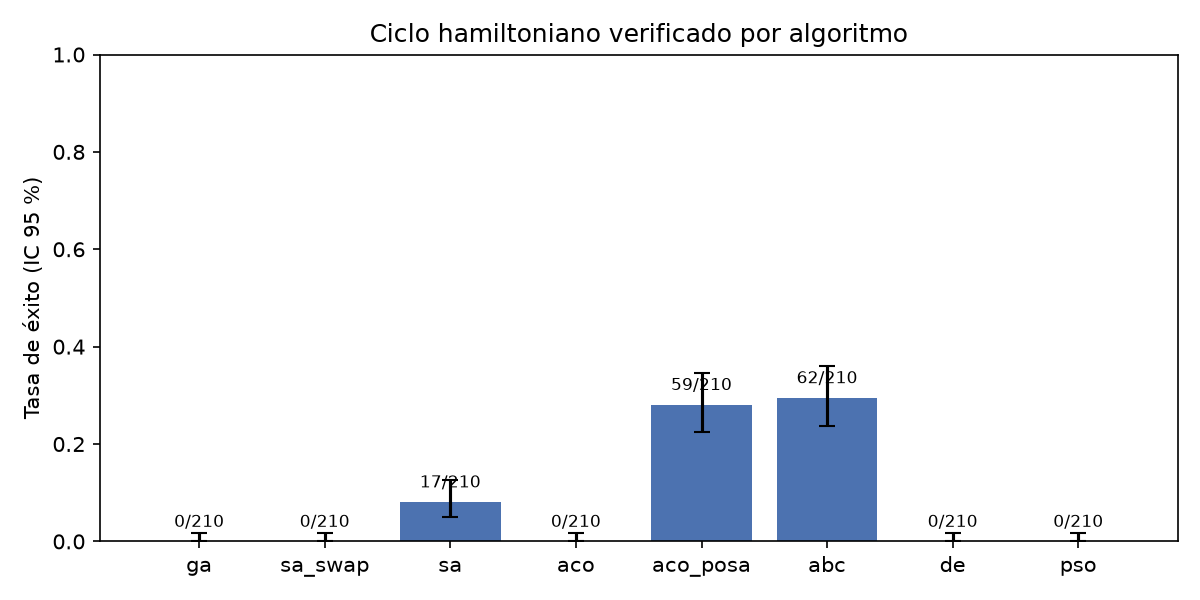
\includegraphics[width=.8\textwidth]{disenoA/exito_algoritmos.png}
\caption{Experimento A: tasa de éxito por algoritmo, con su intervalo de confianza del 95\,\%.}
\label{fig:exitoA}
\end{figure}

En cuanto al tiempo (figura~\ref{fig:tiempoA}), cuando encuentran el ciclo, \alg{ACO + Pósa}
lo hace en 1.2 segundos en la mediana y \alg{ABC} en 3.3 segundos; tres de cada cuatro éxitos
llegan antes de los 15 segundos. \alg{SA (mixto)} es más lento: tarda unos 19 segundos en la
mediana y necesita millones de evaluaciones (unos 2.7 millones) porque pasa la primera parte de la
búsqueda con la temperatura alta.

Como explicamos en la sección~\ref{sec:aco}, el número de evaluaciones de \alg{ACO + Pósa}
(unas 2\,000 en la mediana) no se puede comparar con el de los demás, porque las rotaciones de
Pósa hacen mucho trabajo que no se cuenta como evaluación.

\begin{figure}[H]
\centering
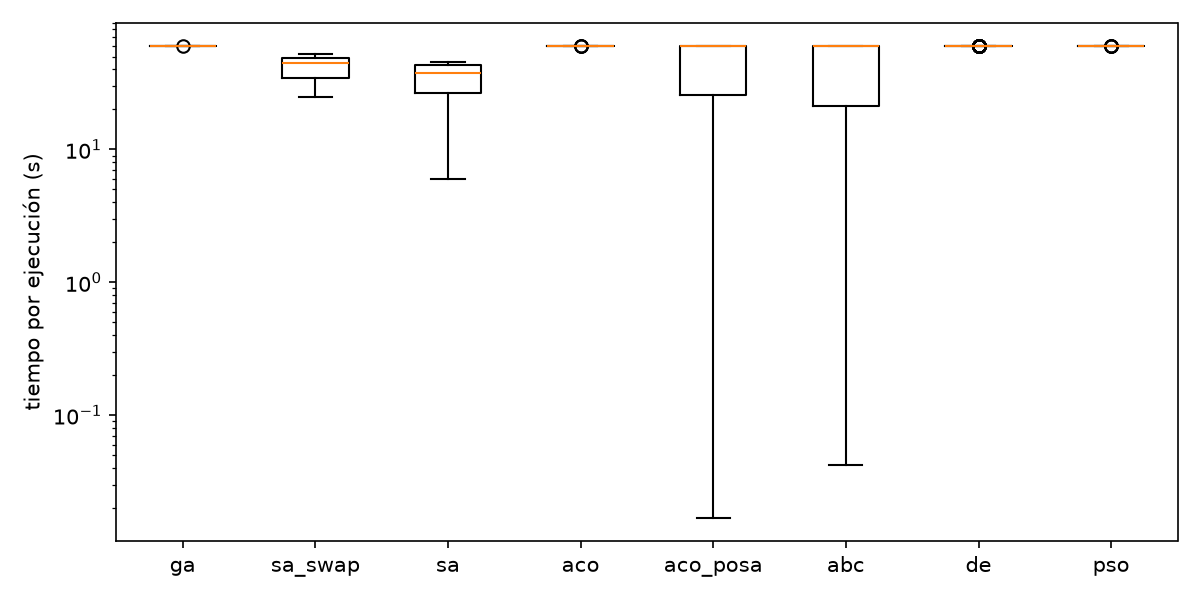
\includegraphics[width=.8\textwidth]{disenoA/tiempo_boxplot.png}
\caption{Experimento A: tiempo de cada corrida (en escala logarítmica).}
\label{fig:tiempoA}
\end{figure}

\section{Resultados por grafo}
Al ver los resultados grafo por grafo (tabla~\ref{tab:instanciasA} y figura~\ref{fig:heatmapA})
se nota que el éxito depende sobre todo del grafo. Cuando \alg{ABC} o \alg{ACO + Pósa} pueden
resolver un grafo, casi siempre lo hacen en las 10 semillas. Y hay 14 de los 21 grafos que ningún
algoritmo pudo resolver ni una vez.

\begin{table}[H]
\centering\small\filas
\caption{Experimento A: corridas exitosas (de 10) por grafo y algoritmo.}
\label{tab:instanciasA}
\resizebox{\textwidth}{!}{% Generado por Reporte/actualizar.py; no editar a mano.
\begin{tabular}{lrrcccccccc}
\toprule
Grafo & $n$ & $m$ & GA & SA (swap) & SA (mixto) & ACO & ACO + Pósa & ABC & DE & PSO \\
\midrule
graph4 & 84 & 127 & 0/10 & 0/10 & 0/10 & 0/10 & \textbf{10/10} & \textbf{9/10} & 0/10 & 0/10 \\
graph5 & 90 & 135 & 0/10 & 0/10 & 0/10 & 0/10 & 0/10 & 0/10 & 0/10 & 0/10 \\
graph6 & 94 & 142 & 0/10 & 0/10 & \textbf{6/10} & 0/10 & \textbf{10/10} & \textbf{10/10} & 0/10 & 0/10 \\
graph7 & 102 & 153 & 0/10 & 0/10 & 0/10 & 0/10 & 0/10 & 0/10 & 0/10 & 0/10 \\
graph8 & 108 & 163 & 0/10 & 0/10 & 0/10 & 0/10 & \textbf{1/10} & \textbf{3/10} & 0/10 & 0/10 \\
graph9 & 114 & 171 & 0/10 & 0/10 & 0/10 & 0/10 & 0/10 & 0/10 & 0/10 & 0/10 \\
graph10 & 118 & 178 & 0/10 & 0/10 & \textbf{4/10} & 0/10 & \textbf{10/10} & \textbf{10/10} & 0/10 & 0/10 \\
graph11 & 126 & 189 & 0/10 & 0/10 & 0/10 & 0/10 & 0/10 & 0/10 & 0/10 & 0/10 \\
graph12 & 132 & 199 & 0/10 & 0/10 & 0/10 & 0/10 & 0/10 & 0/10 & 0/10 & 0/10 \\
graph13 & 138 & 207 & 0/10 & 0/10 & 0/10 & 0/10 & 0/10 & 0/10 & 0/10 & 0/10 \\
graph14 & 142 & 214 & 0/10 & 0/10 & \textbf{3/10} & 0/10 & \textbf{10/10} & \textbf{10/10} & 0/10 & 0/10 \\
graph15 & 150 & 225 & 0/10 & 0/10 & 0/10 & 0/10 & 0/10 & 0/10 & 0/10 & 0/10 \\
graph16 & 156 & 235 & 0/10 & 0/10 & 0/10 & 0/10 & 0/10 & 0/10 & 0/10 & 0/10 \\
graph17 & 162 & 243 & 0/10 & 0/10 & 0/10 & 0/10 & 0/10 & 0/10 & 0/10 & 0/10 \\
graph18 & 166 & 250 & 0/10 & 0/10 & \textbf{3/10} & 0/10 & \textbf{10/10} & \textbf{10/10} & 0/10 & 0/10 \\
graph19 & 170 & 390 & 0/10 & 0/10 & 0/10 & 0/10 & 0/10 & 0/10 & 0/10 & 0/10 \\
graph20 & 174 & 261 & 0/10 & 0/10 & 0/10 & 0/10 & 0/10 & 0/10 & 0/10 & 0/10 \\
graph21 & 180 & 271 & 0/10 & 0/10 & 0/10 & 0/10 & 0/10 & 0/10 & 0/10 & 0/10 \\
graph22 & 186 & 279 & 0/10 & 0/10 & 0/10 & 0/10 & 0/10 & 0/10 & 0/10 & 0/10 \\
graph23 & 190 & 286 & 0/10 & 0/10 & \textbf{1/10} & 0/10 & \textbf{8/10} & \textbf{10/10} & 0/10 & 0/10 \\
graph24 & 198 & 297 & 0/10 & 0/10 & 0/10 & 0/10 & 0/10 & 0/10 & 0/10 & 0/10 \\
\bottomrule
\end{tabular}
}
\end{table}

\begin{figure}[H]
\centering
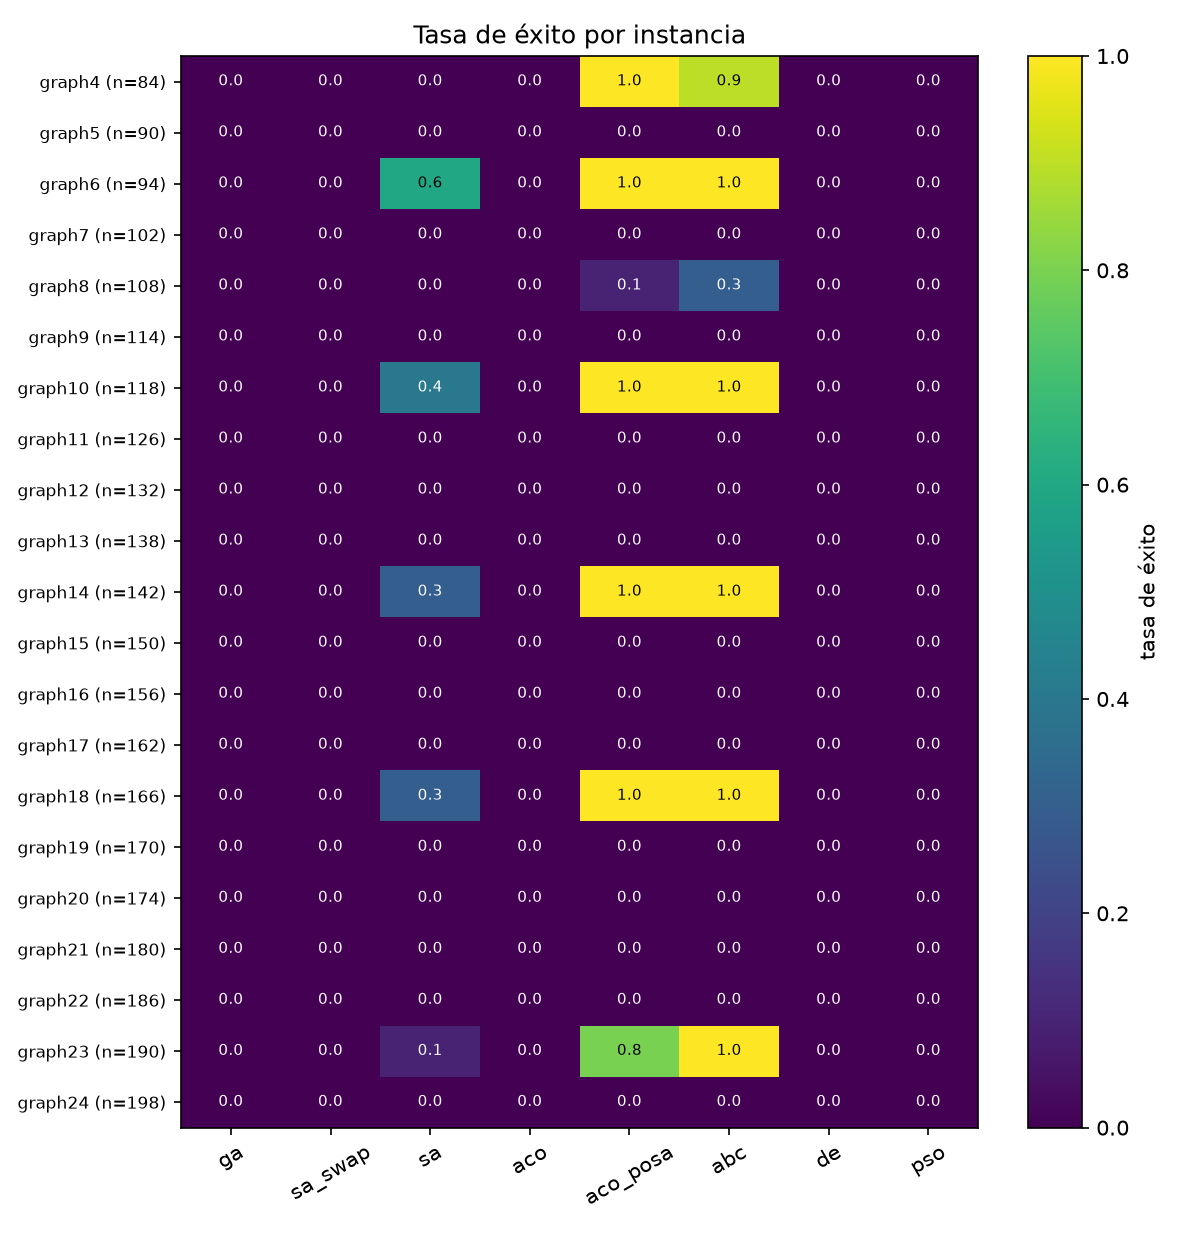
\includegraphics[width=.7\textwidth]{disenoA/heatmap_exito.png}
\caption{Experimento A: tasa de éxito por grafo y algoritmo.}
\label{fig:heatmapA}
\end{figure}

\subsection{Los grafos cúbicos}
Nos preguntamos qué tenían de especial los grafos que nadie resolvió, y al revisar los grados
encontramos un patrón muy claro. Muchos grafos del FHCP son \textbf{cúbicos}: todos sus
vértices tienen exactamente 3 vecinos. Ninguno de los 10 grafos cúbicos del experimento A se
resolvió, y en el experimento B solo se resolvió 1 de 42 (tabla~\ref{tab:cubicos}). En cambio,
los grafos que tienen algunos vértices de grado 4 se resolvieron con mucha más frecuencia.

\begin{table}[H]
\centering\filas
\caption{Grafos resueltos (por cualquier algoritmo) según si son cúbicos o no.}
\label{tab:cubicos}
% Generado por Reporte/actualizar.py; no editar a mano.
\begin{tabular}{lcc}
\toprule
Experimento & Grafos cúbicos resueltos & Grafos no cúbicos resueltos \\
\midrule
A (graph4--graph24) & 0 de 10 & 7 de 11 \\
B (graph1--graph100) & 1 de 42 & 19 de 58 \\
\bottomrule
\end{tabular}

\end{table}

Tiene sentido: con solo 3 vecinos por vértice hay muy pocas formas de entrar y salir de cada uno,
así que casi cualquier decisión equivocada deja a algún vértice sin salida. Esto concuerda con
la idea del FHCP de reunir grafos con estructuras pensadas para ser difíciles \cite{aco8}.

\section{Cómo mejora cada algoritmo (convergencia)}
Las gráficas de convergencia muestran cómo baja el número de aristas faltantes conforme el
algoritmo hace más evaluaciones (figuras~\ref{fig:convA14} y~\ref{fig:convA}). Cada línea es la
mediana de las 10 semillas.

\begin{figure}[H]
\centering
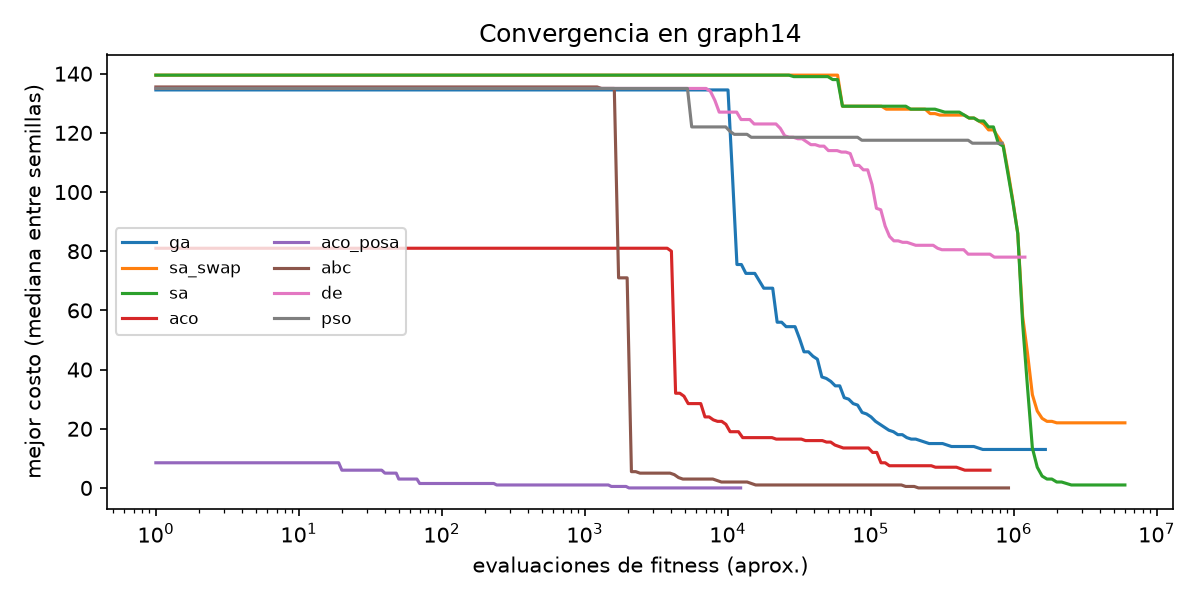
\includegraphics[width=\textwidth]{disenoA/convergencia_graph14.png}
\caption{Experimento A: convergencia en graph14 (142 vértices).}
\label{fig:convA14}
\end{figure}

\begin{figure}[H]
\centering
\begin{subfigure}{.49\textwidth}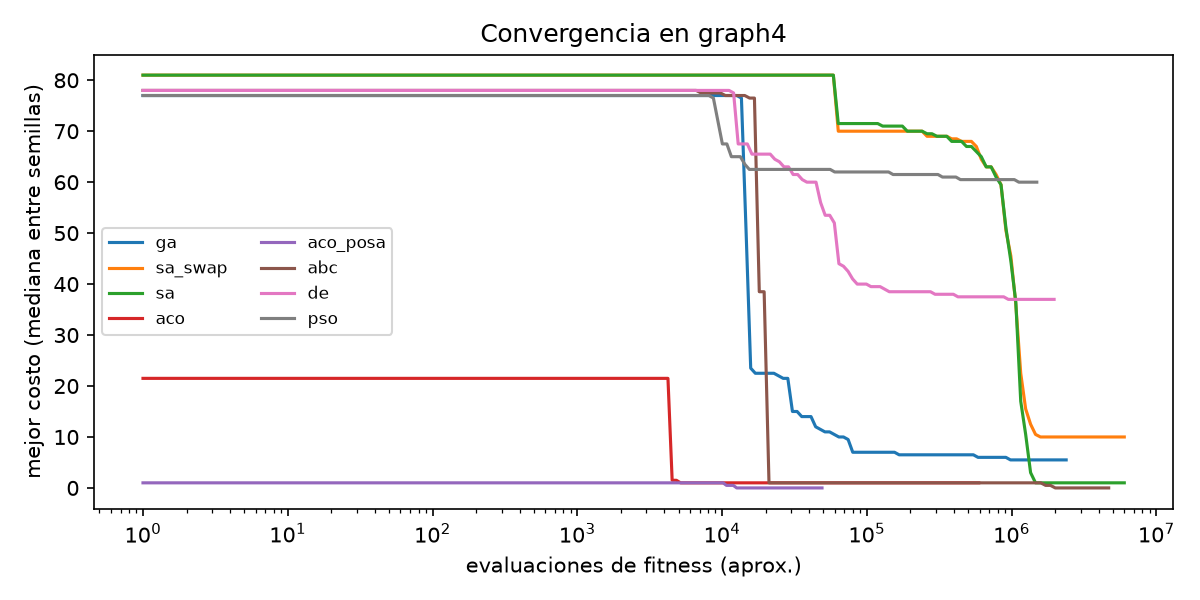
\includegraphics[width=\textwidth]{disenoA/convergencia_graph4.png}\caption{graph4 (84 vértices)}\end{subfigure}
\begin{subfigure}{.49\textwidth}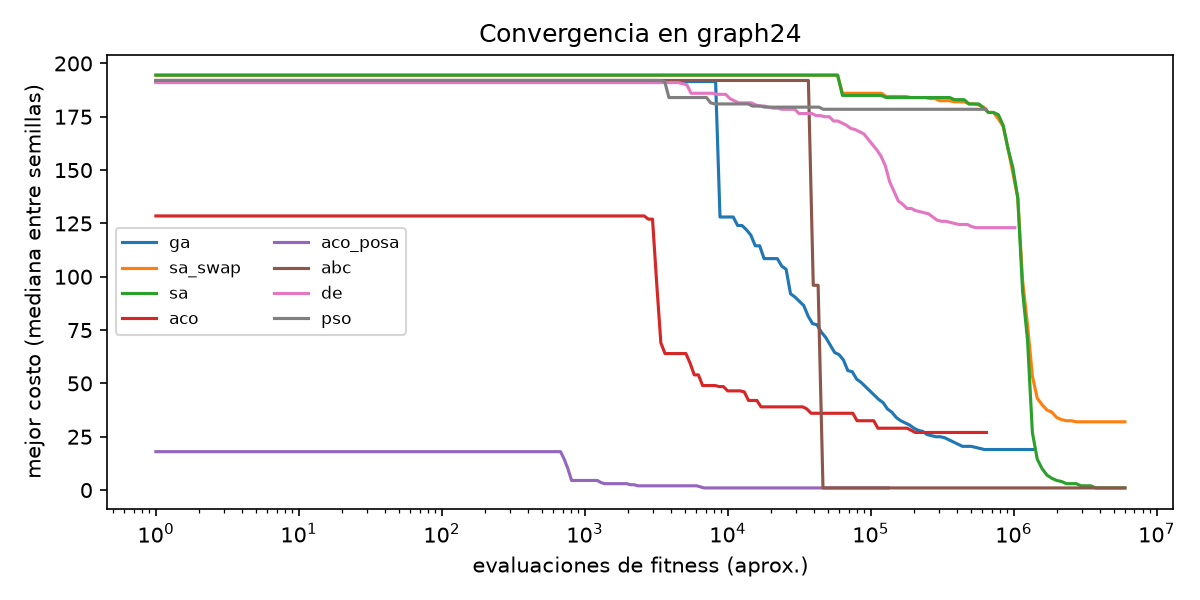
\includegraphics[width=\textwidth]{disenoA/convergencia_graph24.png}\caption{graph24 (198 vértices)}\end{subfigure}
\caption{Experimento A: convergencia en el grafo más pequeño y en el más grande.}
\label{fig:convA}
\end{figure}

Lo que observamos:
\begin{itemize}
  \item \alg{ACO + Pósa} empieza ya muy cerca de la solución, porque las hormigas construyen las
        rutas sobre aristas reales y las rotaciones las alargan.
  \item \alg{ABC} baja de golpe en las primeras miles de evaluaciones, gracias a la inversión
        guiada, y luego afina poco a poco.
  \item \alg{SA} casi no mejora al principio, porque con la temperatura alta acepta muchos cambios
        malos. Ya que se enfría, baja muy rápido y llega cerca de cero, pero tarde.
  \item \alg{GA} y \alg{ACO} sin rotaciones mejoran al principio y luego se estancan.
  \item \alg{DE} y \alg{PSO} apenas mejoran y se quedan con muchas aristas faltantes. Con
        \emph{random keys}, un cambio pequeño en los números puede reordenar media ruta, así que
        al algoritmo le cuesta mucho ir mejorando poco a poco.
\end{itemize}

\section{Qué tan cerca se quedaron}
La figura~\ref{fig:costoA} muestra las aristas faltantes al terminar. Aunque no encontraran el
ciclo, \alg{ABC}, \alg{ACO + Pósa} y \alg{SA (mixto)} se quedaron en promedio a menos de una
arista de la solución. \alg{DE} y \alg{PSO} quedaron muy lejos (79 y 119 aristas faltantes en
promedio).

\begin{figure}[H]
\centering
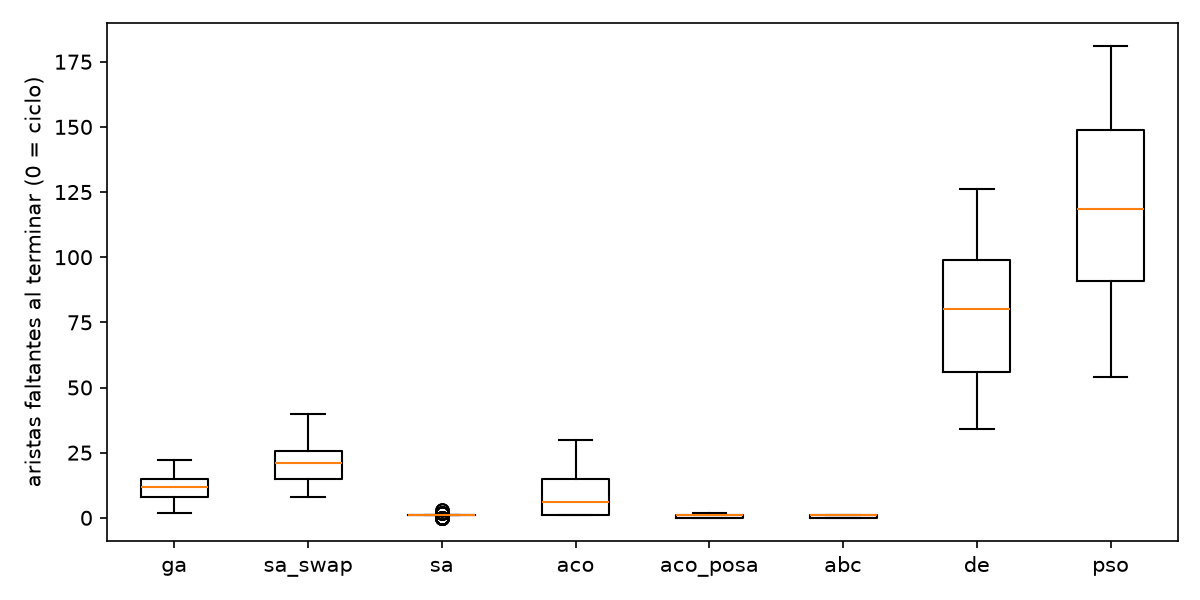
\includegraphics[width=.8\textwidth]{disenoA/costo_final_boxplot.png}
\caption{Experimento A: aristas faltantes al terminar (0 significa que encontró el ciclo).}
\label{fig:costoA}
\end{figure}

\section{Grafos grandes (experimento C)}
En el experimento C probamos los ocho algoritmos con grafos mucho más grandes, con un límite de
2 minutos (tabla~\ref{tab:escalabilidad}). Ninguno encontró un ciclo, pero la diferencia en qué
tan cerca quedaron es enorme. En graph1001, con 9\,528 vértices, a \alg{ABC} le faltaron solo 88
aristas; a \alg{SA (mixto)}, más de 9\,000, y \alg{DE} y \alg{PSO} quedaron prácticamente igual que
una ruta al azar. En graph50 (348 vértices), a \alg{ABC} y a \alg{SA (mixto)} les faltó
\emph{una sola arista}.

\begin{table}[H]
\centering\small\filas
\caption{Experimento C: aristas faltantes al terminar. En negritas, el mejor resultado de cada grafo (una semilla, \tiempoC\,s).}
\label{tab:escalabilidad}
\resizebox{\textwidth}{!}{% Generado por Reporte/actualizar.py; no editar a mano.
\begin{tabular}{lrrrrrrrrrr}
\toprule
Grafo & $n$ & $m$ & GA & SA (swap) & SA (mixto) & ACO & ACO + Pósa & ABC & DE & PSO \\
\midrule
graph50 & 348 & 523 & 35 & 51 & \textbf{1} & 97 & 7 & \textbf{1} & 253 & 323 \\
graph200 & 1200 & 1902 & 649 & 284 & 76 & 579 & 369 & \textbf{9} & 1167 & 1182 \\
graph500 & 2915 & 7271 & 2385 & 995 & 585 & 2549 & 1462 & \textbf{21} & 2889 & 2897 \\
graph1001 & 9528 & 13968 & 9436 & 5806 & 9087 & 8806 & 7201 & \textbf{88} & 9515 & 9516 \\
\bottomrule
\end{tabular}
}
\end{table}

\begin{figure}[H]
\centering
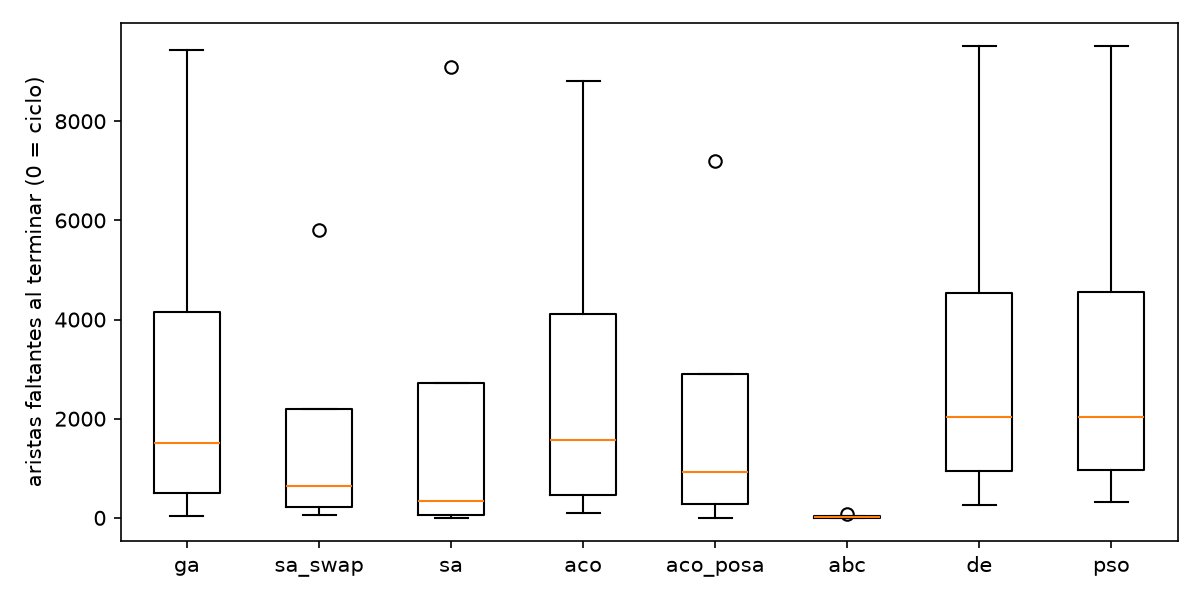
\includegraphics[width=.8\textwidth]{disenoC/costo_final_boxplot.png}
\caption{Experimento C: aristas faltantes al terminar.}
\label{fig:costoC}
\end{figure}

Si vemos las aristas faltantes como porcentaje del total de vértices, \alg{ABC} se mantiene por
debajo del 1\,\% incluso en el grafo más grande, mientras que los demás algoritmos empeoran
mucho conforme crece el grafo. Es decir, \alg{ABC} es el único que escala razonablemente bien.

\chapter{Comparación con el FHCP Challenge}
\label{cap:bench}

\section{El FHCP Challenge}
El FHCP Challenge Set fue publicado por el Flinders Hamiltonian Cycle Project, de la Universidad
Flinders en Australia \cite{aco8,aco9}. Tiene 1\,001 grafos de entre 66 y 9\,528 vértices (en
promedio, poco más de 3\,000), y de todos se sabe que tienen ciclo hamiltoniano.

Con este conjunto se organizó un concurso del 30 de septiembre de 2015 al 30 de septiembre de
2016. Las reglas, según la página oficial \cite{aco9}, eran:
\begin{itemize}
  \item Las soluciones se entregaban en el formato TOUR, el mismo que usamos nosotros.
  \item Una solución contaba solo si era un ciclo hamiltoniano válido.
  \item Ganaba quien resolviera los 1\,001 grafos o, si nadie lo lograba, quien resolviera más.
        En caso de empate, ganaba quien hubiera entregado primero.
  \item El premio era de 1\,001 dólares.
\end{itemize}

Nadie resolvió los 1\,001 grafos. Los ganadores fueron Nathann Cohen y David Coudert, que
encontraron ciclos hamiltonianos en \textbf{985 grafos} \cite{aco9}.

Para nuestro trabajo tomamos el mismo criterio de éxito (un ciclo verificado) y el mismo formato
de salida. La diferencia es que nosotros comparamos con las \emph{soluciones oficiales} que publica
el proyecto, una para cada grafo.

\section{Calidad de las soluciones}
En este problema, una solución es correcta o no lo es: no hay ciclos hamiltonianos ``mejores''
que otros. Todas las soluciones que encontraron nuestros algoritmos las guardamos en formato TOUR
y pasaron el mismo verificador que acepta las soluciones oficiales
(sección~\ref{sec:verificacion}). Así que, en los grafos que resolvimos, nuestra solución es tan
válida como la oficial. En los que no resolvimos, lo que podemos reportar es cuántas aristas
faltaron.

\section{Grafos resueltos (experimento B)}
En el experimento B corrimos \alg{ABC} y \alg{ACO + Pósa} sobre los primeros 100 grafos del
conjunto, con 2 semillas y 2 minutos por corrida (tabla~\ref{tab:benchmarking}).

\begin{table}[H]
\centering\small\filas
\caption{Experimento B: grafos resueltos en al menos una de las \semillasB{} semillas, comparados con las soluciones oficiales.}
\label{tab:benchmarking}
\resizebox{\textwidth}{!}{% Generado por Reporte/actualizar.py; no editar a mano.
\begin{tabular}{lrrrrr}
\toprule
Instancias & $n$ & ACO + Pósa & ABC & Cualquiera de los dos & Con solución oficial \\
\midrule
graph1--graph25 & 66--204 & 9 & 8 & 9 & 25 \\
graph26--graph50 & 210--348 & 0 & 6 & 6 & 25 \\
graph51--graph75 & 354--468 & 0 & 2 & 2 & 25 \\
graph76--graph100 & 471--558 & 0 & 3 & 3 & 25 \\
\midrule
Total & & 9 & 19 & 20 & 100 \\
\bottomrule
\end{tabular}
}
\end{table}

\alg{ABC} resolvió \resueltasBABC{} de los \grafosB{} grafos y \alg{ACO + Pósa},
\resueltasBACOposa{}. Juntos resolvieron 20, porque 8 de los 9 grafos que resolvió
\alg{ACO + Pósa} también los resolvió \alg{ABC} (la excepción es graph1). La diferencia más importante es el tamaño:
\alg{ACO + Pósa} no resolvió ningún grafo después de graph25 (más de 204 vértices), mientras que
\alg{ABC} siguió resolviendo algunos hasta los 558 vértices.

\begin{table}[H]
\centering\filas
\caption{Experimento B: resumen por algoritmo.}
\label{tab:resumenB}
\resizebox{\textwidth}{!}{% Generado por Reporte/actualizar.py; no editar a mano.
\begin{tabular}{lrcrrrrr}
\toprule
Algoritmo & Éxitos & Tasa de éxito [IC 95\,\%] & Grafos resueltos & Tiempo (s) & Evaluaciones hasta el éxito & Aristas faltantes (prom.) & F1 \\
\midrule
ACO + Pósa & 14/200 & 0.07 [0.04, 0.11] & 9/100 & 112.5 $\pm$ 28.7 & 1\,281 & 30.54 & 0.13 \\
ABC & 30/200 & 0.15 [0.11, 0.21] & 19/100 & 105.7 $\pm$ 35.9 & 291\,682 & 2.50 & 0.26 \\
\bottomrule
\end{tabular}
}
\end{table}

\begin{figure}[H]
\centering
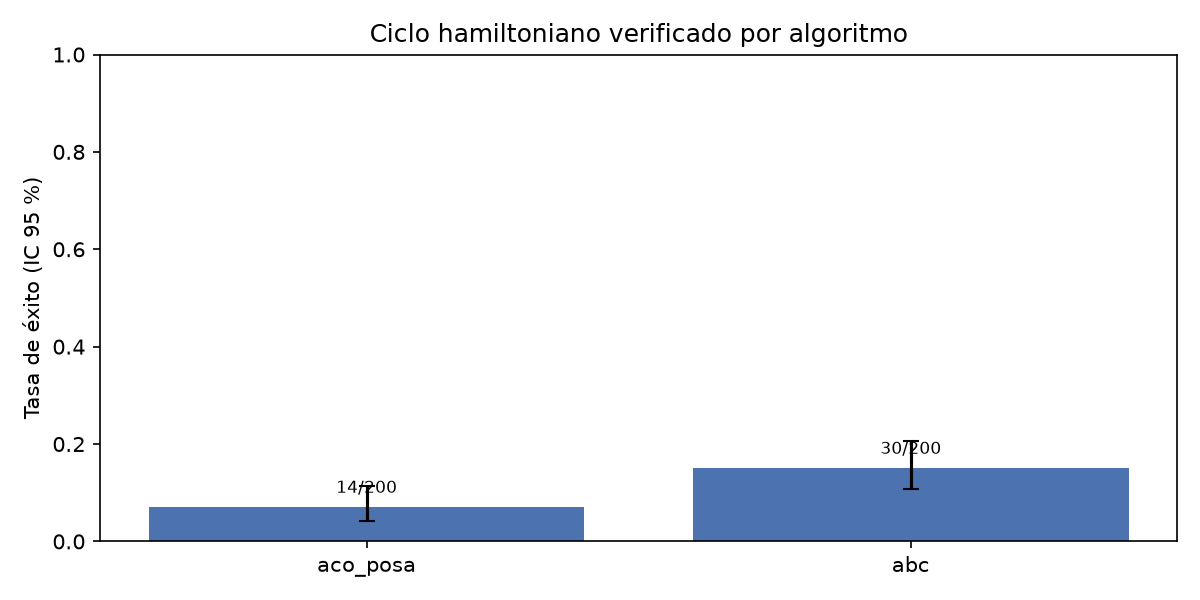
\includegraphics[width=.7\textwidth]{disenoB/exito_algoritmos.png}
\caption{Experimento B: tasa de éxito por algoritmo.}
\label{fig:exitoB}
\end{figure}

Los grafos que resolvió cada algoritmo fueron:
% Generado por Reporte/actualizar.py; no editar a mano.
\begin{description}
\item[ACO + Pósa] graph1, graph2, graph4, graph6, graph8, graph10, graph14, graph18, graph23.
\item[ABC] graph2, graph4, graph6, graph8, graph10, graph14, graph18, graph23, graph27, graph31, graph35, graph39, graph43, graph47, graph52, graph67, graph78, graph85, graph99.
\end{description}


\begin{figure}[H]
\centering
\begin{subfigure}{.49\textwidth}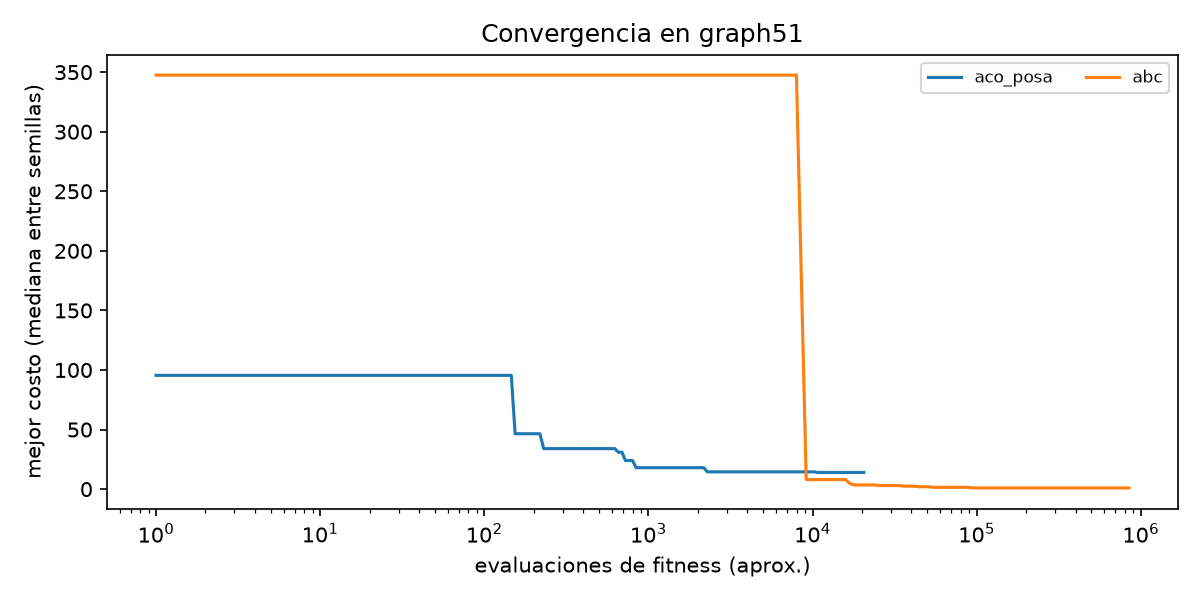
\includegraphics[width=\textwidth]{disenoB/convergencia_graph51.png}\caption{graph51}\end{subfigure}
\begin{subfigure}{.49\textwidth}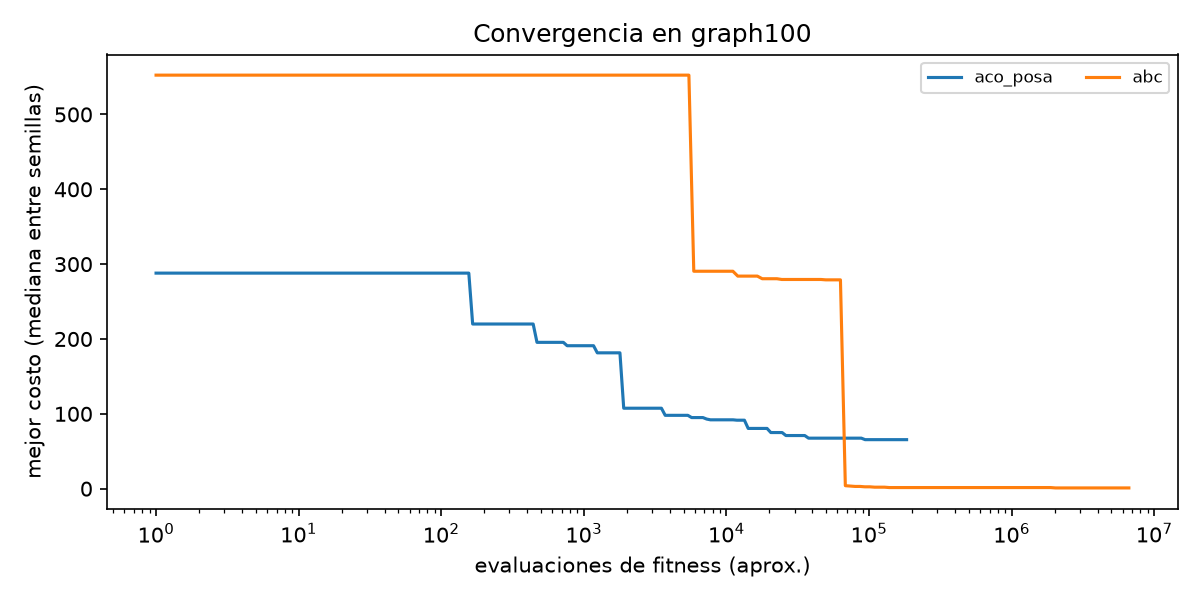
\includegraphics[width=\textwidth]{disenoB/convergencia_graph100.png}\caption{graph100}\end{subfigure}
\caption{Experimento B: convergencia en dos grafos medianos.}
\label{fig:convB}
\end{figure}

\section{Nuestros resultados frente a los mejores}
La diferencia con los mejores resultados es grande. Los ganadores del concurso resolvieron 985 de
los 1\,001 grafos, incluidos los más grandes. Nosotros, en los 100 grafos más pequeños, resolvimos
20 en total. Creemos que esta diferencia se explica por tres razones:
\begin{enumerate}
  \item \textbf{Algoritmos especializados.} Los mejores métodos para este problema están
        diseñados específicamente para ciclos hamiltonianos o para el TSP. Un ejemplo es la
        heurística \emph{Snakes and Ladders}, desarrollada por el mismo grupo de investigación del
        FHCP \cite{slh2014}. Otro es convertir el problema en un TSP y resolverlo con programas como
        LKH \cite{lkh2000}, que tienen búsquedas locales muy potentes. Nuestras metaheurísticas son
        de uso general.
  \item \textbf{Tiempo de cómputo.} Nosotros dimos 2 minutos por corrida. Un concurso de un año
        permite usar horas o días por grafo.
  \item \textbf{Implementación.} Nuestro código está en Python puro, que es bastante más lento que
        el C o C++ que suelen usar estas herramientas.
\end{enumerate}

Aun así, nuestros resultados dejan una lección clara: los dos algoritmos que mejor funcionaron
son los que buscan aprovechando la estructura del grafo (aristas reales, reparaciones locales y
rotaciones), que es también la idea en la que se basan los métodos especializados.

\chapter{Conclusiones}
\label{cap:concl}

\section{¿Qué metaheurística funcionó mejor?}
La que mejor se adaptó a los grafos difíciles del FHCP fue la \textbf{colonia artificial de abejas
(ABC)}. Tuvo la tasa de éxito más alta en el experimento A (empatada con \alg{ACO + Pósa}),
en el benchmarking resolvió más del doble de grafos que \alg{ACO + Pósa}
(\resueltasBABC{} de \grafosB{}, contra \resueltasBACOposa) y fue la que quedó más cerca de la solución en los grafos grandes,
con menos del 1\,\% de aristas faltantes incluso con 9\,528 vértices.

La \textbf{colonia de hormigas con rotaciones de Pósa} fue igual de buena en los grafos pequeños,
y a veces más rápida, pero no escaló: a partir de unos 200 vértices dejó de resolver grafos.

\section{Lo que aprendimos}
\begin{enumerate}
  \item \textbf{La representación y los movimientos importan más que el algoritmo.} Los tres
        algoritmos con éxito usan información del grafo para moverse: ABC repara conexiones con
        aristas reales, ACO camina solo por aristas que existen y usa rotaciones, y SA (mixto)
        invierte tramos. Los que se mueven a ciegas (GA, SA con intercambios) o sobre números
        reales (DE y PSO) no encontraron ningún ciclo.
  \item \textbf{Un cambio pequeño puede hacer una gran diferencia.} SA solo con intercambios no
        resolvió nada, pero con la mitad de los movimientos cambiados a inversiones logró
        \exitosASA{} éxitos con el mismo presupuesto. Lo mismo pasó con ACO: sin rotaciones, 0
        éxitos; con rotaciones, \exitosAACOposa.
  \item \textbf{Las random keys no funcionan bien para este problema.} Garantizan rutas válidas,
        pero un cambio pequeño en las claves puede reordenar media ruta, así que DE y PSO casi no
        pueden mejorar poco a poco. En los grafos grandes quedaron prácticamente igual que una
        ruta al azar.
  \item \textbf{Los grafos cúbicos son el gran cuello de botella.} Casi ninguno se resolvió
        (solo 1 de los 42 grafos cúbicos que hay entre los primeros 100). Con solo tres vecinos por vértice, cualquier error
        deja vértices sin salida.
  \item \textbf{No encontrar el ciclo no significa que no exista.} Todos los grafos del FHCP
        tienen ciclo hamiltoniano, así que cada corrida sin éxito es un límite de nuestros
        algoritmos, no del grafo.
\end{enumerate}

\section{Limitaciones}
\begin{itemize}
  \item La comparación fue a igual tiempo y no a igual número de evaluaciones
        (tabla~\ref{tab:presupuesto}), así que algunos algoritmos usaron muchas más evaluaciones
        que otros.
  \item Las rotaciones de Pósa no se cuentan como evaluaciones, lo que hace que \alg{ACO + Pósa}
        parezca más barato de lo que es.
  \item Usamos los parámetros iniciales de cada algoritmo, sin una calibración sistemática sobre el
        FHCP. Es posible que GA, DE o PSO mejoren con otros valores.
  \item En el experimento B usamos 2 semillas por grafo y en el C solo una, así que esos resultados
        son menos seguros que los del experimento A.
  \item El código está en Python puro, así que los tiempos no se pueden comparar directamente con
        los de herramientas escritas en C o C++.
\end{itemize}

\section{Trabajo futuro}
\begin{itemize}
  \item Calibrar los parámetros de cada algoritmo con algunos grafos reservados para eso.
  \item Agregar a DE y PSO un paso de búsqueda local con la inversión guiada, para ver si así
        logran competir.
  \item Dar más tiempo a los grafos que no se resolvieron, en especial a los cúbicos.
  \item Combinar lo mejor de ABC y de ACO + Pósa: construir rutas con hormigas y luego mejorarlas
        con abejas.
\end{itemize}


\appendix
\chapter{Código fuente y cómo ejecutarlo}
\label{anx:codigo}

El código está en el repositorio del equipo. Necesita Python 3.10 o superior. Los algoritmos y
los experimentos solo usan la biblioteca estándar; para las gráficas se necesitan
\texttt{matplotlib} y \texttt{numpy}, que vienen en \texttt{requirements.txt}.

\section{Resolver un grafo}
\begin{verbatim}
python -m src datos/fhcp/graph4.hcp --alg abc --semilla 0
python -m src datos/fhcp/graph4.hcp --alg aco_posa --tour g4.tour
python -m src --listar        # muestra los algoritmos disponibles
\end{verbatim}
El programa carga el grafo, ejecuta la metaheurística y muestra el arreglo de vértices de la
ruta (numerados de 1 a $n$). Si termina con código 0, encontró un ciclo y lo verificó; si termina
con 1, la corrida quedó inconclusa.

\section{Repetir los experimentos y este reporte}
\begin{verbatim}
python -m venv .venv
source .venv/bin/activate          # en fish: source .venv/bin/activate.fish
pip install -r requirements.txt
bash datos/descargar_fhcp.sh       # descarga los 1001 grafos (para B y C)
python -m src.experimentos A --procesos 16     # igual para B y C
python -m src.graficas resultados/disenoA.jsonl
python Reporte/actualizar.py       # pasa tablas y figuras al reporte
cd Reporte && latexmk -pdf main.tex
\end{verbatim}
Si un experimento se interrumpe, basta con volver a lanzar el mismo comando: continúa donde se
quedó.

\section{Archivos principales}
\begin{table}[H]
\centering\small\filas
\begin{tabularx}{\textwidth}{lL}
\toprule
Archivo & Qué contiene \\
\midrule
\texttt{src/grafo.py} & Lectura de grafos HCP y lectura y escritura de rutas TOUR \\
\texttt{src/fitness.py} & Función de costo, cálculo rápido de cambios y verificación del ciclo \\
\texttt{src/representacion.py} & Conversión de \emph{random keys} a ruta (para DE y PSO) \\
\texttt{src/operadores.py} & Inversión guiada por el grafo \\
\texttt{src/algoritmos/} & GA, SA, ACO, ABC, DE y PSO \\
\texttt{src/experimentos.py} & Ejecución de los experimentos A, B y C en paralelo \\
\texttt{src/graficas.py} & Tablas y gráficas a partir de los resultados \\
\texttt{pruebas/} & Pruebas automáticas de cada parte \\
\texttt{Reporte/} & Este documento \\
\bottomrule
\end{tabularx}
\end{table}


\clearpage
\phantomsection
\addcontentsline{toc}{chapter}{Referencias}
\renewcommand{\bibname}{Referencias}
\begin{thebibliography}{99}
\bibitem{aco1}
M.~Dorigo, V.~Maniezzo y A.~Colorni. «Ant System: Optimization by a colony of
        cooperating agents». IEEE Trans. Systems, Man, and Cybernetics, Part B,
        26(1):29--41, 1996.
        \url{https://doi.org/10.1109/3477.484436}\\
        Respalda: regla de transición probabilística, evaporación y depósito del
        Ant System.

\bibitem{aco2}
M.~Dorigo y L.~M.~Gambardella. «Ant Colony System: A cooperative learning approach to
        the traveling salesman problem». IEEE Trans. Evolutionary Computation,
        1(1):53--66, 1997.
        \url{https://doi.org/10.1109/4235.585892}\\
        Respalda: variante ACS, actualización local y parámetro $q_0$.

\bibitem{aco3}
M.~Dorigo y T.~Stützle. Ant Colony Optimization. MIT Press, 2004.
        \url{https://mitpress.mit.edu/9780262042192/ant-colony-optimization/}\\
        Respalda: visión general de ACO, estigmergia, MMAS, valores de parámetros
        recomendados para el TSP y combinación con búsqueda local.

\bibitem{aco4}
P.~Larrañaga, C.~M.~H.~Kuijpers, R.~H.~Murga, I.~Inza y S.~Dizdarevic. «Genetic
        algorithms for the travelling salesman problem: A review of representations and
        operators». Artificial Intelligence Review, 13(2):129--170, 1999.
        \url{https://doi.org/10.1023/A:1006529012972}\\
        Respalda: representaciones de rutas (camino, adyacencia, ordinal) y su
        efecto en la búsqueda.

\bibitem{aco5}
C.~A.~Coello Coello. «Theoretical and numerical constraint-handling techniques used
        with evolutionary algorithms: a survey of the state of the art».
        Computer Methods in Applied Mechanics and Engineering, 191(11--12):1245--1287,
        2002. \url{https://doi.org/10.1016/S0045-7825(01)00323-1}\\
        Respalda: clasificación de técnicas para manejar restricciones (penalización,
        reparación, operadores que preservan factibilidad).

\bibitem{aco6}
T.~H.~Cormen, C.~E.~Leiserson, R.~L.~Rivest y C.~Stein. Introduction to
        Algorithms, 3.ª ed., MIT Press, 2009, sección 22.1.
        ISBN 978-0-262-03384-8.\\
        Respalda: definiciones de grafo y representaciones por matriz y por listas
        de adyacencia, con sus costos.

\bibitem{aco7}
R.~M.~Karp. «Reducibility among combinatorial problems». En Complexity of
        Computer Computations, pp.~85--103, Plenum Press, 1972.
        \url{https://doi.org/10.1007/978-1-4684-2001-2_9}\\
        Respalda: el ciclo hamiltoniano es NP-completo.

\bibitem{aco8}
M.~Haythorpe. «FHCP Challenge Set: The first set of structurally difficult instances
        of the Hamiltonian cycle problem». Bulletin of the ICA, 83:98--107, 2018.
        \url{https://arxiv.org/abs/1902.10352}\\
        Respalda: 1001 instancias hamiltonianas cuya dificultad proviene de la
        estructura, no solo del tamaño.

\bibitem{aco9}
Flinders Hamiltonian Cycle Project. «FHCP Challenge Set» (sitio oficial).
        \url{https://sites.flinders.edu.au/flinders-hamiltonian-cycle-project/fhcp-challenge-set/}\\
        Respalda: rango de 66 a 9528 vértices, formato HCP y TOUR, resultado del
        concurso (985 de 1001 grafos resueltos por el equipo ganador).

\bibitem{aco10}
L.~Pósa. «Hamiltonian circuits in random graphs». Discrete Mathematics,
        14(4):359--364, 1976. \url{https://doi.org/10.1016/0012-365X(76)90068-6}\\
        Respalda: técnica de rotación para extender caminos hacia ciclos hamiltonianos.

\bibitem{aco11}
J.~C.~Bean. «Genetic algorithms and random keys for sequencing and optimization».
        ORSA Journal on Computing, 6(2):154--160, 1994.
        \url{https://doi.org/10.1287/ijoc.6.2.154}\\
        Respalda: representación por llaves aleatorias.

\bibitem{aco12}
I.~A.~Wagner y A.~M.~Bruckstein. «Hamiltonian(t) -- An ant-inspired heuristic for
        recognizing Hamiltonian graphs». Proc. Congress on Evolutionary Computation
        (CEC 99), 1999. \url{https://doi.org/10.1109/CEC.1999.782656}\\
        Respalda: antecedente de hormigas aplicadas específicamente al ciclo
        hamiltoniano.

\bibitem{aco13}
T.~Stützle y H.~H.~Hoos. «MAX--MIN Ant System». Future Generation Computer
        Systems, 16(8):889--914, 2000.
        \url{https://doi.org/10.1016/S0167-739X(00)00043-1}\\
        Respalda: depósito solo de la mejor hormiga y límites de feromona.

\bibitem{abc1}
Flinders Hamiltonian Cycle Project, ``Flinders Hamiltonian Cycle Project'', s.~f., \url{https://sites.flinders.edu.au/flinders-hamiltonian-cycle-project/}. Define el problema hamiltoniano y distingue su objetivo del TSP. El equipo del proyecto, ``FHCP Challenge Set'', s.~f., \url{https://sites.flinders.edu.au/flinders-hamiltonian-cycle-project/fhcp-challenge-set/}, describe el conjunto FHCP y su formato. Se citan como fuente institucional de contexto, no como evidencia experimental de este ejemplo.

\bibitem{abc2}
Michael Haythorpe, ``FHCP Challenge Set: The First Set of Structurally Difficult Instances of the Hamiltonian Cycle Problem'', 2018, \url{https://arxiv.org/abs/1902.10352}. Respalda la identidad y finalidad del conjunto FHCP. La fecha de publicación del artículo de revista es 2018; la versión arXiv enlazada es posterior.

\bibitem{abc3}
David L. Poole y Alan K. Mackworth, Artificial Intelligence: Foundations of Computational Agents, 3.\textsuperscript{a} ed., Cambridge University Press, 2023, sección 3.6, \url{https://www.artint.info/3e/html/ArtInt3e.Ch3.S6.html}. Respalda la explicación de búsqueda informada y de función heurística como guía estimativa.

\bibitem{abc4}
John H. Holland, Adaptation in Natural and Artificial Systems, 1975; reimpresión MIT Press, 1992, \url{https://doi.org/10.7551/MITPRESS/1090.001.0001}. Fundamento histórico del algoritmo genético y de la adaptación mediante recombinación y selección.

\bibitem{abc5}
Xin-She Yang, ``Metaheuristic Optimization'', Scholarpedia, 2011, \url{https://www.scholarpedia.org/article/Metaheuristic_Optimization}. Respalda el esquema general de GA: codificación, fitness, población, selección, cruce, mutación y reemplazo.

\bibitem{abc6}
David E. Goldberg y Robert Lingle Jr., ``Alleles, Loci, and the Traveling Salesman Problem'', Proceedings of the First International Conference on Genetic Algorithms, 1985, \url{https://gpbib.pmacs.upenn.edu/icga/icga1985-ocr.pdf}. Respalda el uso de permutaciones y cruces especializados, como PMX, para recorridos.

\bibitem{abc7}
Derviş Karaboğa, ``An Idea Based on Honey Bee Swarm for Numerical Optimization'', informe técnico TR06, Universidad de Erciyes, 2005, \href{https://citeseerx.ist.psu.edu/document?doi=cf20e34a1402a115523910d2a4243929f6704db1&repid=rep1&type=pdf}{enlace al informe}. Fuente primaria de las fases de ABC, roles de abejas, fuentes, selección y parámetro \texttt{limit}.

\bibitem{abc8}
Derviş Karaboğa, ``Artificial Bee Colony Algorithm'', Scholarpedia 5(3):6915, 2010, \href{https://www.scholarpedia.org/article/Artificial_bee_colony_algorithm}{enlace al artículo}. Expone la versión de ABC con selección probabilística, mejora voraz, abandono y controles principales.

\bibitem{abc9}
Indadul Khan y Manas Kumar Maiti, ``A Swap Sequence Based Artificial Bee Colony Algorithm for Traveling Salesman Problem'', Swarm and Evolutionary Computation 44, 428--438, 2019, \url{https://doi.org/10.1016/j.swevo.2018.05.006}. Respalda que las variantes discretas para recorridos requieren operadores de permutación; no se atribuye a este artículo la adaptación específica propuesta aquí.

\bibitem{de1}
Richard M. Karp, ``Reducibility Among Combinatorial Problems'', en Miller y Thatcher (eds.), Complexity of Computer Computations, Plenum, 85--103, 1972, \url{https://people.irisa.fr/Nicolas.Markey/biblio/ccc1972-Kar}. Marco clásico de NP-completitud. Trabajo antiguo y vigente; se verificó la referencia, y queda pendiente confirmar el pasaje específico en el texto.

\bibitem{de2}
Michael Haythorpe, ``FHCP Challenge Set: The First Set of Structurally Difficult Instances of the Hamiltonian Cycle Problem'', Bulletin of the ICA 83, 98--107, 2018, \url{https://arxiv.org/abs/1902.10352}. Fuente primaria sobre la composición y dificultad del conjunto, y sobre la adaptación de algoritmos del TSP.

\bibitem{de3}
Flinders Hamiltonian Cycle Project, ``FHCP Challenge Set'', consultado en noviembre de 2026, \url{https://sites.flinders.edu.au/flinders-hamiltonian-cycle-project/fhcp-challenge-set/}. Página oficial: tamaños, existencia de ciclo en todas las instancias y resultados del concurso.

\bibitem{de4}
Joeri Sleegers y Daan van den Berg, ``Looking for the Hardest Hamiltonian Cycle Problem Instances'', ECTA 2020, 40--48, 2020, \url{https://doi.org/10.5220/0010066900400048}. Respalda la relación entre densidad y facilidad. Artículo de congreso.

\bibitem{de5}
Thomas Bartz-Beielstein et al., ``Benchmarking in Optimization: Best Practice and Open Issues'', arXiv:2007.03488v2, 2020, \url{https://arxiv.org/abs/2007.03488}. Revisión amplia de 17 autores sobre esfuerzo, éxito, fallos, PAR-$k$, resumen de ejecuciones y semillas. Es un preprint sin arbitraje confirmado.

\bibitem{de6}
Nikolaus Hansen, Anne Auger, Dimo Brockhoff, Dejan Tušar y Tea Tušar, ``COCO: Performance Assessment'', arXiv:1605.03560, 2016, \url{https://arxiv.org/abs/1605.03560}. Respalda las evaluaciones como medida, el objetivo fijo, el tratamiento de fallos y el aRT. Su contexto es la optimización continua, de modo que aplicarlo aquí es una transferencia.

\bibitem{de7}
A. E. Eiben y J. E. Smith, Introduction to Evolutionary Computing, 2.\textsuperscript{a} ed., Springer, 2015, \url{https://doi.org/10.1007/978-3-662-44874-8}. Respalda eficiencia, efectividad y la advertencia sobre generaciones. Solo se revisaron \href{https://cin.ufpe.br/~aluizioa/CE/CE-07-trabalhando-com-AEs-ch09-2014.pdf}{diapositivas del capítulo}; el libro queda pendiente.

\bibitem{de8}
Lawrence D. Brown, T. Tony Cai y Anirban DasGupta, ``Interval Estimation for a Binomial Proportion'', Statistical Science 16(2), 101--133, 2001, \url{https://doi.org/10.1214/ss/1009213286}. Respalda la incertidumbre de una tasa de éxito. Se revisó el resumen.

\bibitem{de9}
Peter Christen, David J. Hand y Nishadi Kirielle, ``A Review of the F-Measure: Its History, Properties, Criticism, and Alternatives'', ACM Computing Surveys 56(3), artículo 73, 2023, \url{https://doi.org/10.1145/3606367}. Respalda definiciones y críticas de precisión, recall y F1. Trata la clasificación; no se le atribuye la aplicación al ciclo hamiltoniano hecha aquí.

\bibitem{de10}
Rainer Storn y Kenneth Price, ``Differential Evolution: A Simple and Efficient Heuristic for Global Optimization over Continuous Spaces'', Journal of Global Optimization 11, 341--359, 1997, \href{https://www.cp.eng.chula.ac.th/~piak/teaching/ec/ec2012/storn_price_de.pdf}{copia consultada}. Fuente primaria del algoritmo, la notación y los parámetros. El DOI queda pendiente de confirmar.

\bibitem{de11}
Swagatam Das, Sankha Subhra Mullick y P. N. Suganthan, ``Recent Advances in Differential Evolution: An Updated Survey'', Swarm and Evolutionary Computation 27, 1--30, 2016, \url{https://doi.org/10.1016/j.swevo.2016.01.004}. Respalda el desarrollo de DE y la adaptación de parámetros. Se revisó el resumen.

\bibitem{de12}
Karin Zielinski, Petra Weitkemper, Rainer Laur y Karl-Dirk Kammeyer, ``Examination of Stopping Criteria for Differential Evolution based on a Power Allocation Problem'', 10th International Conference on Optimization of Electrical and Electronic Equipment, 2006, \url{https://www.ant.uni-bremen.de/sixcms/media.php/102/4605/ICO3E_2006_zielinski.pdf}. Respalda la clasificación de criterios de paro. Un congreso y un solo problema.

\bibitem{de13}
James C. Bean, ``Genetic Algorithms and Random Keys for Sequencing and Optimization'', ORSA Journal on Computing 6(2), 154--160, 1994, \url{https://doi.org/10.1287/ijoc.6.2.154}. Origen de las claves aleatorias, propuestas para algoritmos genéticos. Se revisó el resumen.

\bibitem{de14}
Pavel Krömer, Vojtěch Uher y Václav Snášel, ``Novel Random Key Encoding Schemes for the Differential Evolution of Permutation Problems'', IEEE Transactions on Evolutionary Computation 26(1), 43--57, 2022, \url{https://doi.org/10.1109/TEVC.2021.3087802}. Respalda el uso de claves aleatorias en DE y en el TSP. Se revisó el resumen.

\bibitem{de15}
Valentino Santucci, Marco Baioletti y Alfredo Milani, ``Algebraic Differential Evolution Algorithm for the Permutation Flowshop Scheduling Problem with Total Flowtime Criterion'', IEEE Transactions on Evolutionary Computation 20(5), 682--694, 2016, \url{https://doi.org/10.1109/TEVC.2015.2507785}. Respalda la crítica a las claves aleatorias y la DE algebraica, en otro problema.

\bibitem{de16}
Godfrey C. Onwubolu y Donald Davendra (eds.), Differential Evolution: A Handbook for Global Permutation-Based Combinatorial Optimization, Springer, 2009, ISBN 978-3-540-92150-9, \url{https://www.wolfram.com/books/profile.cgi?id=7359}. Respalda la existencia de varios enfoques. Solo se revisaron la ficha y el índice.

\bibitem{de17}
Fatih Tasgetiren, Angela Chen, Gunes Gencyilmaz y Said Gattoufi, ``Smallest Position Value Approach'', capítulo 5 de \cite{de16}, 2009, \url{https://www.academia.edu/3714507/Smallest_Position_Value_Approach}. Respalda el uso de SPV con DE en un TSP generalizado. Se revisó un extracto; el detalle de la regla queda pendiente.
\bibitem{sa1} Leighton, T. y Rubinfeld, R. (2006). Mathematics for Computer Science: Notes for Recitation 6. MIT. Definiciones de grafos, recorridos y longitud. \url{https://web.mit.edu/neboat/Public/6.042/rec6.pdf}.
\bibitem{sa2} Diestel, R. (2025). Graph Theory, 6.ª ed. Springer, capítulo 10. Definiciones hamiltonianas; referencia conservada de la investigación de SA. \url{https://www.math.uni-hamburg.de/home/diestel/books/graph.theory/preview/Ch10.pdf}.
\bibitem{sa3} Universidad de Waterloo. The Traveling Salesman Problem. Definición del TSP. \url{https://www.math.uwaterloo.ca/tsp/problem/index.html}.
\bibitem{sa4} Kirkpatrick, S., Gelatt, C. D. y Vecchi, M. P. (1983). Optimization by Simulated Annealing. Science 220(4598), 671--680. Fundamento de SA. \url{https://doi.org/10.1126/science.220.4598.671}.
\bibitem{sa5} Hajek, B. (1988). Cooling Schedules for Optimal Annealing. Mathematics of Operations Research 13(2), 311--329. Condiciones de convergencia. \url{https://doi.org/10.1287/moor.13.2.311}.
\bibitem{sa7} Komosinski, M. Optimization: Simulated annealing. Poznan University of Technology. Material docente citado por el documento original para el pseudocódigo y el enfriamiento. \url{https://www.cs.put.poznan.pl/mkomosinski/lectures/optimization/SA-en.pdf}.
\bibitem{sa8} Metropolis, N., Rosenbluth, A. W., Rosenbluth, M. N., Teller, A. H. y Teller, E. (1953). Equation of State Calculations by Fast Computing Machines. Journal of Chemical Physics 21(6), 1087--1092. Antecedente de la aceptación probabilística. \url{https://doi.org/10.1063/1.1699114}.
\bibitem{pso1995} Kennedy, J. y Eberhart, R. (1995). Particle swarm optimization. Proceedings of ICNN'95, vol. 4, 1942--1948. Fuente original de PSO. \url{https://doi.org/10.1109/ICNN.1995.488968}.
\bibitem{pso1998} Shi, Y. y Eberhart, R. (1998). A modified particle swarm optimizer. IEEE International Conference on Evolutionary Computation, 69--73. Variante con peso de inercia. \url{https://doi.org/10.1109/ICEC.1998.699146}.
% --- Añadidas para el reporte de la Fase 4 (verificar los datos antes de entregar) ---
\bibitem{wilson1927} Wilson, E. B. (1927). Probable Inference, the Law of Succession, and Statistical Inference. Journal of the American Statistical Association 22(158), 209--212. Intervalo de confianza usado para la tasa de éxito. \url{https://doi.org/10.1080/01621459.1927.10502953}.
\bibitem{posa1976} Pósa, L. (1976). Hamiltonian circuits in random graphs. Discrete Mathematics 14(4), 359--364. Rotaciones usadas en la variante ACO + Pósa. \url{https://doi.org/10.1016/0012-365X(76)90068-6}.
\bibitem{slh2014} Baniasadi, P., Ejov, V., Filar, J. A., Haythorpe, M. y Rossomakhine, S. (2014). Deterministic ``Snakes and Ladders'' Heuristic for the Hamiltonian cycle problem. Mathematical Programming Computation 6(1), 55--75. Heurística de referencia del grupo FHCP. \url{https://doi.org/10.1007/s12532-013-0059-2}.
\bibitem{lkh2000} Helsgaun, K. (2000). An effective implementation of the Lin--Kernighan traveling salesman heuristic. European Journal of Operational Research 126(1), 106--130. Base de LKH, usada para resolver instancias del HCP como TSP. \url{https://doi.org/10.1016/S0377-2217(99)00284-2}.

\end{thebibliography}

\end{document}
